% Select document class: uncomment one of the following
\documentclass[aspectratio=169]{beamer}  % For presentation mode
%\documentclass[11pt]{article}            % For article mode
%\usepackage{beamerarticle}               % Uncomment with article class

% =============================================================================
% COMMON PREAMBLE
% =============================================================================
% =============================================================================
% Common Preamble for Network+ Lecture Series
% This file provides consistent formatting, colors, packages, and styles
% across all lecture modules for both beamer presentations and article mode
% =============================================================================

% =============================================================================
% THEME AND COLORS
% =============================================================================
\usetheme{Madrid}
\usecolortheme{whale}

% Custom colors - standardized across all lectures
\definecolor{rctcblue}{RGB}{0, 74, 136}
\definecolor{rctcgold}{RGB}{255, 199, 44}
\definecolor{networkgreen}{RGB}{0, 128, 64}
\definecolor{alertred}{RGB}{180, 0, 0}
\definecolor{aborange}{RGB}{230, 126, 34}
\definecolor{copperbrown}{RGB}{184, 115, 51}
\definecolor{faborange}{RGB}{255, 165, 0}
\definecolor{fiberyellow}{RGB}{255, 215, 0}
\definecolor{shirepurple}{RGB}{102, 51, 153}
\definecolor{ipblue}{RGB}{52, 152, 219}
\definecolor{ippurple}{RGB}{155, 89, 182}
\definecolor{vlangreen}{RGB}{39, 174, 96}
\definecolor{tcpblue}{RGB}{30, 100, 180}
\definecolor{udpgreen}{RGB}{50, 160, 80}
\definecolor{dhcppurple}{RGB}{120, 60, 160}
\definecolor{dnsyellow}{RGB}{200, 170, 50}
\definecolor{batblack}{RGB}{30, 30, 40}
\definecolor{gothamgray}{RGB}{80, 85, 95}
\definecolor{paddysgreen}{RGB}{19, 77, 33}
\definecolor{beerlight}{RGB}{255, 199, 44}
\definecolor{sunnyorange}{RGB}{255, 140, 0}
\definecolor{ogregreen}{RGB}{34, 139, 34}
\definecolor{swampbrown}{RGB}{101, 67, 33}

% Set theme colors
\setbeamercolor{palette primary}{bg=rctcblue,fg=white}
\setbeamercolor{palette secondary}{bg=rctcblue!80,fg=white}
\setbeamercolor{palette tertiary}{bg=rctcblue!60,fg=white}
\setbeamercolor{structure}{fg=rctcblue}
\setbeamercolor{title}{fg=white,bg=rctcblue}
\setbeamercolor{frametitle}{fg=white,bg=rctcblue}
\setbeamercolor{block title}{bg=rctcblue,fg=white}
\setbeamercolor{block body}{bg=rctcblue!10,fg=black}
\setbeamercolor{block title alerted}{bg=alertred,fg=white}
\setbeamercolor{block body alerted}{bg=alertred!10,fg=black}
\setbeamercolor{block title example}{bg=networkgreen,fg=white}
\setbeamercolor{block body example}{bg=networkgreen!10,fg=black}

% =============================================================================
% PACKAGES
% =============================================================================
\usepackage[utf8]{inputenc}
\usepackage[T1]{fontenc}
\usepackage{lmodern}  % Better font rendering
\usepackage{graphicx}
\usepackage{tikz}
\usepackage{booktabs}
\usepackage{array}
\usepackage{multirow}
\usepackage{hyperref}
\usepackage{adjustbox}
\usepackage{amssymb}
\usepackage{amsmath}
\usepackage{calc}
\usepackage{fontawesome5}
% xcolor with [table] option: avoid colortbl.4ht hook conflict in tex4ht
\ifdefined\HCode
  \usepackage{xcolor}
  \usepackage{colortbl}  % provides \rowcolor etc.
\else
  \usepackage[table]{xcolor}  % includes colortbl for pdflatex
\fi

% =============================================================================
% TIKZ LIBRARIES AND SETUP
% =============================================================================
\usetikzlibrary{
    shapes.geometric,
    shapes.symbols,
    shapes.misc,
    arrows.meta,
    positioning,
    calc,
    fit,
    backgrounds,
    decorations.pathreplacing,
    decorations.pathmorphing,
    matrix,
    chains
}
% shadows library causes pgfuseshading errors with tex4ht;
% only load it when NOT building HTML
\ifdefined\HCode\else
    \usetikzlibrary{shadows}
\fi

% Graphics path for icons and chapter images
\graphicspath{
    {../images/icons/}
    {./images/icons/}
    {images/icons/}
    {../images/ch1/}
    {./images/ch1/}
    {images/ch1/}
    {../images/ch2/}
    {./images/ch2/}
    {images/ch2/}
    {../images/ch3/}
    {./images/ch3/}
    {images/ch3/}
    {../images/ch4/}
    {./images/ch4/}
    {images/ch4/}
    {../images/ch5/}
    {./images/ch5/}
    {images/ch5/}
    {../images/ch6/}
    {./images/ch6/}
    {images/ch6/}
    {../images/ch7/}
    {./images/ch7/}
    {images/ch7/}
    {../images/ch8/}
    {./images/ch8/}
    {images/ch8/}
    {../images/ch9/}
    {./images/ch9/}
    {images/ch9/}
    {../images/}
    {./images/}
    {images/}
}

% =============================================================================
% NETWORK DIAGRAM STYLES
% =============================================================================
\tikzset{
    % Node styles for network devices
    device/.style={
        inner sep=2pt,
        label distance=2pt
    },
    pc/.style={device},
    laptop/.style={device},
    server/.style={device},
    router/.style={device},
    switch/.style={device},
    firewall/.style={device},
    cloud/.style={device},
    phone/.style={device},
    tablet/.style={device},
    wifi/.style={device},
    % Connection styles
    ethernet/.style={
        draw=rctcblue,
        line width=1.5pt,
        -{Stealth[length=3mm]}
    },
    ethernet noarrow/.style={
        draw=rctcblue,
        line width=1.5pt
    },
    wireless/.style={
        draw=aborange,
        line width=1.5pt,
        dashed,
        -{Stealth[length=3mm]}
    },
    wireless noarrow/.style={
        draw=aborange,
        line width=1.5pt,
        dashed
    },
    wan/.style={
        draw=alertred,
        line width=2pt,
        -{Stealth[length=3mm]}
    },
    wan noarrow/.style={
        draw=alertred,
        line width=2pt
    },
    copper/.style={
        draw=copperbrown,
        line width=2pt,
        -{Stealth[length=3mm]}
    },
    copper noarrow/.style={
        draw=copperbrown,
        line width=2pt
    },
    fiber/.style={
        draw=fiberyellow,
        line width=2pt,
        -{Stealth[length=3mm]}
    },
    fiber noarrow/.style={
        draw=fiberyellow,
        line width=2pt
    },
    trunk/.style={
        draw=shirepurple,
        line width=2pt,
        -{Stealth[length=3mm]}
    },
    trunk noarrow/.style={
        draw=shirepurple,
        line width=2pt
    },
    % Packet/segment styles
    pktseg/.style={
        draw=rctcblue,
        fill=rctcblue!10,
        minimum height=0.5cm,
        font=\tiny,
        rounded corners=2pt
    },
    pktseg tcp/.style={
        draw=tcpblue,
        fill=tcpblue!15,
        minimum height=0.5cm,
        font=\tiny,
        rounded corners=2pt
    },
    pktseg udp/.style={
        draw=udpgreen,
        fill=udpgreen!15,
        minimum height=0.5cm,
        font=\tiny,
        rounded corners=2pt
    },
    pktseg highlight/.style={
        draw=aborange,
        fill=aborange!20,
        minimum height=0.5cm,
        font=\tiny,
        rounded corners=2pt
    },
    % Box styles
    ipbox/.style={
        draw=rctcblue,
        fill=rctcblue!10,
        rounded corners,
        minimum height=0.4cm,
        font=\small
    },
    portbox/.style={
        draw=tcpblue,
        fill=tcpblue!10,
        rounded corners,
        minimum height=0.4cm,
        font=\small
    },
    dnsbox/.style={
        draw=dnsyellow,
        fill=dnsyellow!15,
        rounded corners,
        minimum height=0.4cm,
        font=\small
    },
    routetable/.style={
        draw=rctcblue,
        fill=rctcblue!10,
        rounded corners,
        minimum height=0.4cm,
        font=\small
    },
    macbox/.style={
        draw=networkgreen,
        fill=networkgreen!10,
        rounded corners,
        minimum height=0.4cm,
        font=\small
    },
    % Frame segment styles (Ethernet frame diagrams)
    frameseg/.style={
        draw=rctcblue,
        fill=rctcblue!10,
        minimum height=0.5cm,
        font=\tiny,
        rounded corners=2pt
    },
    frameseg highlight/.style={
        draw=aborange,
        fill=aborange!20,
        minimum height=0.5cm,
        font=\tiny,
        rounded corners=2pt
    },
    % Process/flow styles
    process/.style={
        draw=rctcblue,
        fill=rctcblue!15,
        rounded corners,
        minimum width=2cm,
        minimum height=0.6cm,
        font=\small,
        align=center
    },
    decision/.style={
        draw=aborange,
        fill=aborange!15,
        diamond,
        aspect=2,
        minimum width=1.5cm,
        font=\small,
        align=center
    },
    % OSI Layer styles
    osilayer/.style={
        draw=rctcblue,
        fill=rctcblue!10,
        minimum width=3cm,
        minimum height=0.45cm,
        font=\small
    },
    osilayer highlight/.style={
        draw=aborange,
        fill=aborange!20,
        line width=1.5pt,
        minimum width=3cm,
        minimum height=0.45cm,
        font=\small\bfseries
    }
}

% =============================================================================
% ICON COMMANDS - Standardized using PNG files and FontAwesome
% =============================================================================
% Network device icons (PNG)
\newcommand{\iconpc}[1][0.6cm]{\resizebox{#1}{!}{
\includegraphics{icon_pc}}}
\newcommand{\iconlaptop}[1][0.6cm]{\resizebox{#1}{!}{
\includegraphics{icon_laptop}}}
\newcommand{\iconserver}[1][0.6cm]{\resizebox{#1}{!}{
\includegraphics{icon_server}}}
\newcommand{\iconrouter}[1][0.6cm]{\resizebox{#1}{!}{
\includegraphics{icon_router}}}
\newcommand{\iconswitch}[1][0.6cm]{\resizebox{#1}{!}{
\includegraphics{icon_switch}}}
\newcommand{\iconfirewall}[1][0.6cm]{\resizebox{#1}{!}{
\includegraphics{icon_firewall}}}
\newcommand{\iconcloud}[1][0.6cm]{\resizebox{#1}{!}{
\includegraphics{icon_cloud}}}
\newcommand{\iconphone}[1][0.6cm]{\resizebox{#1}{!}{
\includegraphics{icon_phone}}}
\newcommand{\icontablet}[1][0.6cm]{\resizebox{#1}{!}{
\includegraphics{icon_tablet}}}
\newcommand{\iconwifi}[1][0.6cm]{\resizebox{#1}{!}{
\includegraphics{icon_wifi}}}
\newcommand{\icondatabase}[1][0.6cm]{\resizebox{#1}{!}{
\includegraphics{icon_db}}}
\newcommand{\iconlock}[1][0.6cm]{\resizebox{#1}{!}{
\includegraphics{icon_lock}}}

% For HTML/tex4ht builds: replace PNG icons with FontAwesome5 glyphs.
% dvisvgm embeds font glyphs as vectors but silently ignores em:graph (PNG)
% specials, so PNG icons would be blank in the output SVGs. FA5 glyphs work.
\ifdefined\HCode
  \renewcommand{\iconpc}[1][0.6cm]{\resizebox{#1}{!}{\faIcon{desktop}}}
  \renewcommand{\iconlaptop}[1][0.6cm]{\resizebox{#1}{!}{\faIcon{laptop}}}
  \renewcommand{\iconserver}[1][0.6cm]{\resizebox{#1}{!}{\faIcon{server}}}
  \renewcommand{\iconrouter}[1][0.6cm]{\resizebox{#1}{!}{\faIcon{route}}}
  \renewcommand{\iconswitch}[1][0.6cm]{\resizebox{#1}{!}{\faIcon{network-wired}}}
  \renewcommand{\iconfirewall}[1][0.6cm]{\resizebox{#1}{!}{\faIcon{shield-alt}}}
  \renewcommand{\iconcloud}[1][0.6cm]{\resizebox{#1}{!}{\faIcon{cloud}}}
  \renewcommand{\iconphone}[1][0.6cm]{\resizebox{#1}{!}{\faIcon{mobile-alt}}}
  \renewcommand{\icontablet}[1][0.6cm]{\resizebox{#1}{!}{\faIcon{tablet-alt}}}
  \renewcommand{\iconwifi}[1][0.6cm]{\resizebox{#1}{!}{\faIcon{wifi}}}
  \renewcommand{\icondatabase}[1][0.6cm]{\resizebox{#1}{!}{\faIcon{database}}}
  \renewcommand{\iconlock}[1][0.6cm]{\resizebox{#1}{!}{\faIcon{lock}}}
\fi

% FontAwesome icons
\newcommand{\iconuser}[1][0.6cm]{\resizebox{#1}{!}{\faIcon{user}}}
\newcommand{\iconglobe}[1][0.6cm]{\resizebox{#1}{!}{\faIcon{globe}}}
\newcommand{\iconclock}[1][0.6cm]{\resizebox{#1}{!}{\faIcon{clock}}}
\newcommand{\iconmail}[1][0.6cm]{\resizebox{#1}{!}{\faIcon{envelope}}}
\newcommand{\icondoc}[1][0.6cm]{\resizebox{#1}{!}{\faIcon{file-alt}}}
\newcommand{\iconsearch}[1][0.6cm]{\resizebox{#1}{!}{\faIcon{search}}}
\newcommand{\icontools}[1][0.6cm]{\resizebox{#1}{!}{\faIcon{tools}}}
\newcommand{\iconchart}[1][0.6cm]{\resizebox{#1}{!}{\faIcon{chart-line}}}
\newcommand{\iconalert}[1][0.6cm]{\resizebox{#1}{!}{\faIcon{bell}}}
\newcommand{\iconlog}[1][0.6cm]{\resizebox{#1}{!}{\faIcon{clipboard-list}}}
\newcommand{\iconeye}[1][0.6cm]{\resizebox{#1}{!}{\faIcon{eye}}}
\newcommand{\iconhacker}[1][0.6cm]{\resizebox{#1}{!}{\faIcon{user-secret}}}
\newcommand{\iconkey}[1][0.6cm]{\resizebox{#1}{!}{\faIcon{key}}}
\newcommand{\iconfile}[1][0.6cm]{\resizebox{#1}{!}{\faIcon{file-alt}}}
\newcommand{\icondog}[1][0.6cm]{\resizebox{#1}{!}{\faIcon{dog}}}
\newcommand{\iconcat}[1][0.6cm]{\resizebox{#1}{!}{\faIcon{cat}}}
\newcommand{\iconvoip}[1][0.6cm]{\resizebox{#1}{!}{\faIcon{phone-volume}}}
\newcommand{\iconmoney}[1][0.6cm]{\resizebox{#1}{!}{\faIcon{money-bill-wave}}}
\newcommand{\icontrash}[1][0.6cm]{\resizebox{#1}{!}{\faIcon{trash}}}
\newcommand{\iconbuilding}[1][0.6cm]{\resizebox{#1}{!}{\faIcon{building}}}

% =============================================================================
% CUSTOM COMMANDS AND ENVIRONMENTS
% =============================================================================

% Key term formatting
\newcommand{\keyterm}[1]{\textbf{#1}}

% Slide section marker
\newcommand{\sectionslide}[1]{
    \begin{frame}
        \vfill
        \centering
        \begin{beamercolorbox}[sep=8pt,center,shadow=true,rounded=true]{title}
            \usebeamerfont{title}\Huge #1
        \end{beamercolorbox}
        \vfill
    \end{frame}
}

% Case study frame environment
\newenvironment{casestudy}[1]{%
    \begin{alertblock}{$\blacktriangleright$ Case Study: #1}
}{%
    \end{alertblock}
}

% Solution frame environment  
\newenvironment{casesolution}[1]{%
    \begin{exampleblock}{$\checkmark$ Solution: #1}
}{%
    \end{exampleblock}
}

% =============================================================================
% FOOTER WITH SLIDE NUMBERS
% =============================================================================
\setbeamertemplate{footline}{
    \leavevmode%
    \hbox{%
        \begin{beamercolorbox}[wd=.333333\paperwidth,ht=2.25ex,dp=1ex,center]{author in head/foot}%
            \usebeamerfont{author in head/foot}\insertshortauthor
        \end{beamercolorbox}%
        \begin{beamercolorbox}[wd=.333333\paperwidth,ht=2.25ex,dp=1ex,center]{title in head/foot}%
            \usebeamerfont{title in head/foot}\insertshorttitle
        \end{beamercolorbox}%
        \begin{beamercolorbox}[wd=.333333\paperwidth,ht=2.25ex,dp=1ex,right]{date in head/foot}%
            \usebeamerfont{date in head/foot}\insertshortdate{}\hspace*{2em}
            \insertframenumber{} / \inserttotalframenumber\hspace*{2ex}
        \end{beamercolorbox}}%
    \vskip0pt%
}

% =============================================================================
% ARTICLE MODE SUPPORT
% =============================================================================
% The following commands help with beamerarticle mode for HTML conversion

% In article mode, add proper section/subsection support and override environments
\mode<article>{
    % Make sure figure captions work properly
    \setbeamertemplate{caption}[numbered]
    \setbeamertemplate{caption label separator}{: }
    
    % Add some spacing for readability
    \setlength{\parskip}{0.5em}
    \setlength{\parindent}{0pt}
    
    % Article mode versions of case study environments
    \renewenvironment{casestudy}[1]{%
        \vspace{0.3cm}\noindent\textbf{Case Study: #1}\newline\begin{itshape}
    }{%
        \end{itshape}\vspace{0.3cm}
    }
    
    \renewenvironment{casesolution}[1]{%
        \vspace{0.3cm}\noindent\textbf{Solution: #1}\newline\begin{itshape}
    }{%
        \end{itshape}\vspace{0.3cm}
    }
}

% Command to mark content that only appears in article mode
\newcommand{\articleonly}[1]{\mode<article>{#1}}

% Command to mark content that only appears in presentation mode
\newcommand{\presentationonly}[1]{\mode<presentation>{#1}}


% =============================================================================
% DOCUMENT INFO
% =============================================================================
\title[Network+ Module 3.0]{Network Interfaces and Switches}
\subtitle{Network+ Module 3.0}
\author[B. Shea]{Brendan Shea, PhD}
\institute[RCTC]{Rochester Community and Technical College\\Intro to Networking}
\date{}

\mode<article>{
\let\originaltikzpicture\tikzpicture
\let\endoriginaltikzpicture\endtikzpicture
\renewenvironment{tikzpicture}[1][]{%
    \originaltikzpicture[#1]%
}{%
    \endoriginaltikzpicture%
    \par\small\emph{Figure: Diagram supporting the preceding content.}\par
}
}

\begin{document}

% =============================================================================
% SLIDE 1: Title Slide
% =============================================================================
\begin{frame}
    \titlepage
    \begin{center}
        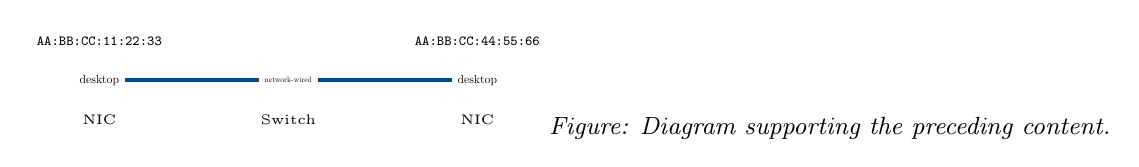
\begin{tikzpicture}[scale=0.8]
            % NIC to Switch connection illustration
            \node[pc] (pc1) at (0,0) {\iconpc[0.5cm]};
            \node[font=\tiny, below] at (0,-0.4) {NIC};
            
            \node[switch] (sw) at (3,0) {\iconswitch[0.6cm]};
            \node[font=\tiny, below] at (3,-0.4) {Switch};
            
            \node[pc] (pc2) at (6,0) {\iconpc[0.5cm]};
            \node[font=\tiny, below] at (6,-0.4) {NIC};
            
            % Connections
            \draw[ethernet noarrow] (pc1) -- (sw);
            \draw[ethernet noarrow] (sw) -- (pc2);
            
            % MAC addresses
            \node[font=\tiny, above] at (0,0.4) {\texttt{AA:BB:CC:11:22:33}};
            \node[font=\tiny, above] at (6,0.4) {\texttt{AA:BB:CC:44:55:66}};
        \end{tikzpicture}
    \end{center}
\end{frame}

% Table of contents in presentation mode only
\presentationonly{
\begin{frame}[allowframebreaks]{Outline}
\small
\tableofcontents[hideallsubsections]
\end{frame}
}


% =============================================================================
% SLIDE 2: Review - From Cables to Connections
% =============================================================================
\section*{Review from Module 2}

\begin{frame}{Review: From Cables to Connections}
    \begin{columns}[T]
        \begin{column}{0.55\textwidth}
            \begin{itemize}
                \item Module 2 covered \textbf{physical cables}---copper, fiber, and connectors.
                \item Today's question: What do those cables \textit{plug into}?
                \item Two key components:
                    \begin{itemize}
                        \item \keyterm{NICs}---in computers (endpoints)
                        \item \keyterm{Switches}---connecting everything together
                    \end{itemize}
                \item We're moving from Layer 1 (Physical) into Layer 2 (Data Link).
            \end{itemize}
            
            \vspace{0.3em}
            \begin{alertblock}{Layer 2 Focus}
                Cables carry bits, but NICs and switches work with \textbf{frames} and \textbf{MAC addresses}.
            \end{alertblock}
        \end{column}
        \begin{column}{0.42\textwidth}
            \begin{center}
                % CAPTION: OSI model seven layers emphasizing Layer 2 Data Link
                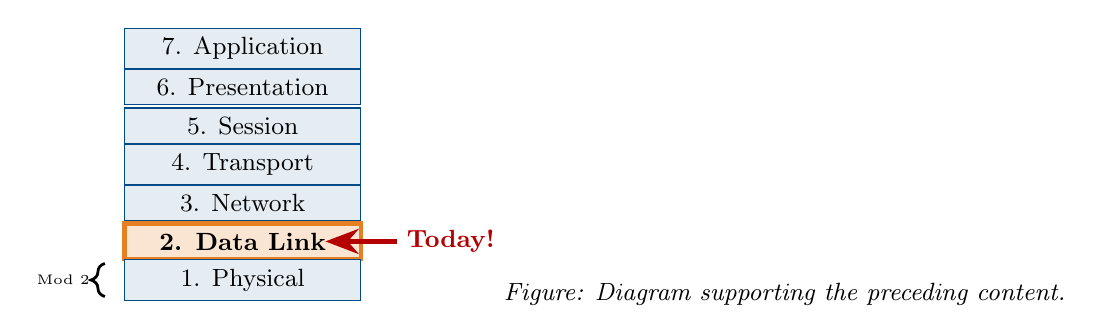
\begin{tikzpicture}[scale=0.7]
                    % OSI Stack
                    \node[osilayer] (l7) at (0, 3.5) {7. Application};
                    \node[osilayer] (l6) at (0, 2.8) {6. Presentation};
                    \node[osilayer] (l5) at (0, 2.1) {5. Session};
                    \node[osilayer] (l4) at (0, 1.4) {4. Transport};
                    \node[osilayer] (l3) at (0, 0.7) {3. Network};
                    \node[osilayer highlight] (l2) at (0, 0) {2. Data Link};
                    \node[osilayer] (l1) at (0, -0.7) {1. Physical};
                    
                    % Arrow pointing to focus
                    \draw[-{Stealth}, line width=2pt, alertred] (2.8, 0) -- (1.5, 0);
                    \node[right, font=\small\bfseries, alertred] at (2.8, 0) {Today!};
                    
                    % Module 2 bracket
                    \draw[decorate, decoration={brace, amplitude=5pt}, line width=1pt] 
                        (-2.5, -1) -- (-2.5, -0.4);
                    \node[left, font=\tiny] at (-2.6, -0.7) {Mod 2};
                \end{tikzpicture}
            \end{center}
        \end{column}
    \end{columns}
\end{frame}

% =============================================================================
% SLIDE 3: Learning Outcomes
% =============================================================================
\begin{frame}[t,allowframebreaks]{Learning Outcomes}
    After completing this module, you will be able to:
    \vspace{0.5em}
    \begin{itemize}
        \item Explain the function of \keyterm{Network Interface Cards (NICs)} and their role in host connectivity.
        \item Identify and describe \keyterm{modular transceivers} including SFP, SFP+, and QSFP.
        \item Interpret \keyterm{MAC addresses} and explain the \keyterm{OUI} (Organizationally Unique Identifier) format.
        \item Describe the structure of an \keyterm{Ethernet frame} and identify its key fields.
        \item Compare and contrast \keyterm{hubs}, \keyterm{bridges}, and \keyterm{switches} as Layer 2 devices.
        \item Explain how switches use \keyterm{MAC address tables} to make forwarding decisions.
        \item Configure basic switch settings including hostnames, IP addresses, and \keyterm{link aggregation}.
        \item Describe advanced switch features including \keyterm{STP}, \keyterm{PoE}, and Layer 3 switching.
        \item Troubleshoot common switch problems using LED indicators, \keyterm{show commands}, and error counters.
    \end{itemize}
\end{frame}



% =============================================================================
% SLIDE 5: What is a Network Interface Card (NIC)?
% =============================================================================
\section{Network Interface Foundations}
\subsection{NIC Fundamentals}

\articleonly{
This section introduces network interfaces and transceivers, the hardware endpoints that connect hosts to Ethernet networks and expose physical and data-link functions.
}

\begin{frame}{What is a Network Interface Card (NIC)?}
    \begin{columns}[T]
        \begin{column}{0.55\textwidth}
            \begin{itemize}
                \item A \keyterm{NIC} is the hardware that connects a computer to the network.
                \item Every NIC has a unique \keyterm{MAC address} burned in at the factory.
                \item NICs translate between computer data and network signals (electrical or optical).
                \item Modern computers usually have NICs built into the motherboard.
            \end{itemize}
            
            \vspace{0.3em}
            \begin{block}{NIC Responsibilities}
                \begin{itemize}
                    \item Create and process Ethernet frames
                    \item Convert data to/from network signals
                    \item Manage link speed and duplex settings
                \end{itemize}
            \end{block}
        \end{column}
        \begin{column}{0.42\textwidth}
            \begin{center}
                % CAPTION: Computer system with NIC hardware for network connectivity
                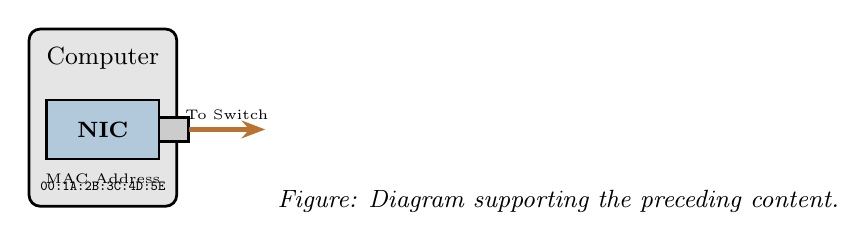
\begin{tikzpicture}[scale=0.75]
                    % Computer
                    \draw[fill=gray!20, line width=1pt, rounded corners] (0,0) rectangle (2.5,3);
                    \node[font=\small] at (1.25, 2.5) {Computer};
                    
                    % NIC inside
                    \draw[fill=rctcblue!30, line width=1pt] (0.3,0.8) rectangle (2.2,1.8);
                    \node[font=\footnotesize\bfseries] at (1.25, 1.3) {NIC};
                    
                    % RJ-45 port
                    \draw[fill=gray!40, line width=1pt] (2.2,1.1) rectangle (2.7,1.5);
                    
                    % Cable going out
                    \draw[copper, line width=2pt] (2.7,1.3) -- (4,1.3);
                    \node[font=\tiny, above] at (3.35, 1.3) {To Switch};
                    
                    % MAC label
                    \node[font=\tiny, align=center] at (1.25, 0.4) {MAC Address\\[-0.5em]\texttt{00:1A:2B:3C:4D:5E}};
                \end{tikzpicture}
            \end{center}
            
            \vspace{0.3em}
            \begin{alertblock}{Key Point}
                Without a NIC, your computer is an island---no network access!
            \end{alertblock}
        \end{column}
    \end{columns}
\end{frame}




% =============================================================================
% SLIDE 6: NIC Examples
% =============================================================================
\begin{frame}{NIC Examples}
    \begin{center}
        \mode<beamer>{
\includegraphics[width=0.8\textwidth]{three_NICs}}
        \articleonly{
\includegraphics[width=0.8\textwidth]{three_NICs}\\
        \small\emph{Figure: Examples of network interface cards with different ports and form factors.}}
    \end{center}
    \begin{center}
        \small
        Examples of different network interface cards showing various form factors and connector types.
    \end{center}
\end{frame}

% =============================================================================
% SLIDE 7: NIC Features and Specifications
% =============================================================================
\begin{frame}{NIC Features and Specifications}
    \begin{columns}[T]
        \begin{column}{0.52\textwidth}
            \begin{itemize}
                \item \textbf{Speed ratings}: 1 Gbps, 10 Gbps, 25 Gbps, 100 Gbps.
                \item \textbf{Connector types}: RJ-45 (copper) or SFP/SFP+ (fiber).
                \item \keyterm{Wake-on-LAN (WoL)}: Start a powered-off computer remotely over the network.
                \item \keyterm{Offloading}: NIC handles checksums, segmentation---reduces CPU load.
                \item Server NICs often have multiple ports.
            \end{itemize}
            
            \vspace{0.3em}
            \begin{exampleblock}{Auto-Negotiation}
                NICs automatically negotiate the best speed and duplex with the switch. Usually ``just works''!
            \end{exampleblock}
        \end{column}
        \begin{column}{0.45\textwidth}
            \begin{center}
                \small
                \begin{tabular}{l l}
                    \toprule
                    \textbf{NIC Type} & \textbf{Typical Use} \\
                    \midrule
                    1 Gbps RJ-45 & Desktops, laptops \\
                    10 Gbps RJ-45 & Workstations \\
                    10 Gbps SFP+ & Servers \\
                    25/100 Gbps & Data centers \\
                    \bottomrule
                \end{tabular}
            \end{center}
            
            \vspace{0.5em}
            \begin{block}{Dual-Port NICs}
                Servers use multiple NIC ports for:
                \begin{itemize}
                    \item Redundancy (failover)
                    \item Increased bandwidth
                    \item Separate networks
                \end{itemize}
            \end{block}
        \end{column}
    \end{columns}
\end{frame}


\begin{frame}{What is a Transceiver?}
    \begin{columns}[T]
        \begin{column}{0.52\textwidth}
            \begin{itemize}
                \item A \keyterm{transceiver} is a device that both \textbf{transmits} and \textbf{receives} signals.
                \item Converts between electrical signals (inside the device) and optical or electrical signals (on the cable).
                \item \keyterm{TX}: Transmit (outgoing signal)
                \item \keyterm{RX}: Receive (incoming signal)
                \item Think of it as a translator between two different ``languages'' of communication.
            \end{itemize}
            
            \vspace{0.3em}
            \begin{block}{Why Transceivers Matter}
                Without a transceiver, your switch can't understand fiber optic light signals---it only speaks electrical!
            \end{block}
        \end{column}
        \begin{column}{0.45\textwidth}
            \begin{center}
                \mode<beamer>{
\includegraphics[width=\textwidth]{transceiver_cutaway}}
                \articleonly{
\includegraphics[width=\textwidth]{transceiver_cutaway}\\
                \small\emph{Figure: Transceiver cutaway showing optical/electrical conversion components.}}
            \end{center}
            
            \vspace{0.3em}
            \begin{alertblock}{Key Components}
                \small
                \textbf{Laser/LED}: Converts electrical $\rightarrow$ light \\
                \textbf{Photodetector}: Converts light $\rightarrow$ electrical \\
                \textbf{Circuit board}: Manages the conversion
            \end{alertblock}
        \end{column}
    \end{columns}
\end{frame}


\begin{frame}[t,shrink=20]{Table: Types of Transceivers}
    \begin{center}
        \scriptsize
        \begin{tabular}{l l l l l}
            \toprule
            \textbf{Transceiver} & \textbf{Speed} & \textbf{Cable Type} & \textbf{Connector} & \textbf{Distance} \\
            \midrule
            SFP & 1 Gbps & MMF or SMF & LC & 550m (MMF) \\
            & & & & 10km (SMF) \\
            \midrule
            SFP+ & 10 Gbps & MMF or SMF & LC & 300m (MMF) \\
            & & & & 10--80km (SMF) \\
            \midrule
            QSFP & 40 Gbps & MMF or SMF & MPO/MTP & 100m (MMF) \\
            & & & & 10km (SMF) \\
            \midrule
            QSFP28 & 100 Gbps & MMF or SMF & MPO/MTP & 100m (MMF) \\
            & & & & 10km (SMF) \\
            \midrule
            GBIC & 1 Gbps & MMF or SMF & SC & 550m (MMF) \\
            (legacy) & & & & 10km (SMF) \\
            \midrule
            SFP-T & 1 Gbps & Copper (UTP) & RJ-45 & 100m \\
            \midrule
            SFP+ DAC & 10 Gbps & Twinax copper & Integrated & 3--7m \\
            \bottomrule
        \end{tabular}
    \end{center}
    
    \vspace{0.2em}
    \centering\scriptsize
    \textbf{MMF} = Multimode Fiber \quad \textbf{SMF} = Single-mode Fiber \quad \textbf{DAC} = Direct Attach Cable.
    \\
    Always match transceiver type to cable type and required distance.
\end{frame}
% =============================================================================
% SLIDE A: Layer 1 Network Diagram - The Green Dragon Physical Infrastructure
% =============================================================================
\begin{frame}{Layer 1: Physical Infrastructure at the Green Dragon}
    \begin{center}
        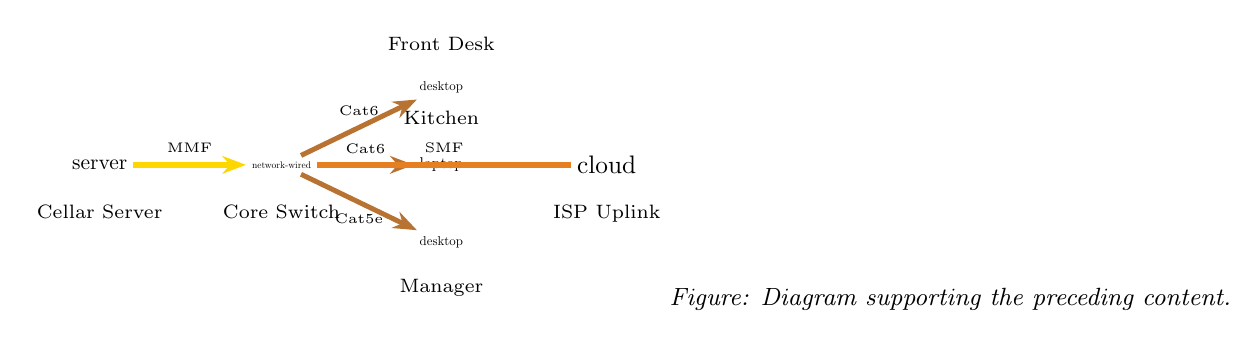
\begin{tikzpicture}[scale=0.7]
            \node[server] (srv) at (0,0) {\iconserver[0.7cm]};
            \node[font=\scriptsize, below] at (0,-0.55) {Cellar Server};

            \node[switch] (sw) at (3.3,0) {\iconswitch[0.75cm]};
            \node[font=\scriptsize, below] at (3.3,-0.55) {Core Switch};

            \node[pc] (pc1) at (6.2,1.4) {\iconpc[0.55cm]};
            \node[font=\scriptsize, above] at (6.2,1.9) {Front Desk};

            \node[laptop] (pc2) at (6.2,0) {\iconlaptop[0.55cm]};
            \node[font=\scriptsize, above] at (6.2,0.55) {Kitchen};

            \node[pc] (pc3) at (6.2,-1.4) {\iconpc[0.55cm]};
            \node[font=\scriptsize, below] at (6.2,-1.9) {Manager};

            \node[cloud] (wan) at (9.2,0) {\iconcloud[0.75cm]};
            \node[font=\scriptsize, below] at (9.2,-0.55) {ISP Uplink};

            \draw[fiber, line width=2pt] (srv) -- node[above, font=\tiny] {MMF} (sw);
            \draw[copper, line width=1.8pt] (sw) -- node[above, font=\tiny] {Cat6} (pc1);
            \draw[copper, line width=1.8pt] (sw) -- node[above, font=\tiny] {Cat6} (pc2);
            \draw[copper, line width=1.8pt] (sw) -- node[below, font=\tiny] {Cat5e} (pc3);
            \draw[draw=aborange, line width=2pt] (sw) -- node[above, font=\tiny] {SMF} (wan);
        \end{tikzpicture}
    \end{center}

    \vspace{0.2em}
    {\centering \scriptsize Layer 1 maps physical links between endpoints, switching infrastructure, and uplinks.\par}
\end{frame}

% =============================================================================
% SLIDE 8: Transceiver Issues
% =============================================================================
\begin{frame}{Transceiver Issues}
    \begin{columns}[T]
        \begin{column}{0.48\textwidth}
            \begin{block}{Mismatch Issues}
                \begin{itemize}
                    \small
                    \item SFP in SFP+ port: May work at reduced speed
                    \item SFP+ in SFP port: \textbf{Won't work}
                    \item Different vendors may be incompatible (some switches are picky!)
                    \item Fiber type mismatch: MMF transceiver + SMF cable = no link
                \end{itemize}
            \end{block}
            
            \vspace{0.3em}
            \begin{alertblock}{Vendor Lock-In}
                Some manufacturers only accept their own branded transceivers. Third-party modules are cheaper but may not work.
            \end{alertblock}
        \end{column}
        \begin{column}{0.48\textwidth}
            \begin{block}{Signal Strength Issues}
                \begin{itemize}
                    \small
                    \item \keyterm{TX power}: How strong the transmit signal is
                    \item \keyterm{RX sensitivity}: Minimum signal the receiver can detect
                    \item Too little power = signal doesn't reach
                    \item Too much power = overwhelms receiver
                \end{itemize}
            \end{block}
            
            \vspace{0.3em}
            \begin{exampleblock}{Troubleshooting Tip: Transceivers}
                \begin{enumerate}
                    \item Transceiver compatibility
                    \item Fiber type (MMF vs SMF)
                    \item Cable distance vs. transceiver rating
                \end{enumerate}
            \end{exampleblock}
        \end{column}
    \end{columns}
\end{frame}

% =============================================================================
% SLIDE 9: Ethernet Frame Format
% =============================================================================
\section{Ethernet Frames and MAC Addressing}
\subsection{Frame Structure and Addressing}

\articleonly{
Here we examine Ethernet frame structure and MAC addressing, which form the basis of Layer 2 switching decisions and local delivery.
}

\begin{frame}{Ethernet Frame Format}
    \begin{itemize}
        \item Data doesn't travel as raw bits---it's packaged into \keyterm{frames}.
        \item Frames contain addressing information so switches know where to send them.
        \item Standard maximum frame size: \textbf{1518 bytes} (or 9000+ for jumbo frames).
    \end{itemize}
    
    \vspace{0.3em}
    \begin{center}
        % CAPTION: Ethernet frame structure showing preamble, MAC addresses, type, payload, and FCS fields
        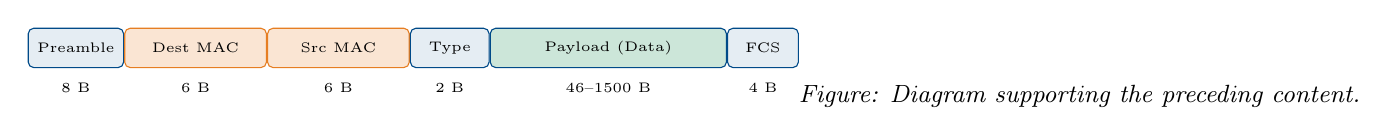
\begin{tikzpicture}[scale=0.85]
            % Frame segments
            \node[frameseg, minimum width=1.2cm] (pre) at (0,0) {Preamble};
            \node[frameseg highlight, minimum width=1.8cm, right=0pt of pre] (dst) {Dest MAC};
            \node[frameseg highlight, minimum width=1.8cm, right=0pt of dst] (src) {Src MAC};
            \node[frameseg, minimum width=1.0cm, right=0pt of src] (type) {Type};
            \node[frameseg, minimum width=3.0cm, right=0pt of type, fill=networkgreen!20] (pay) {Payload (Data)};
            \node[frameseg, minimum width=0.9cm, right=0pt of pay] (fcs) {FCS};
            
            % Size labels below
            \node[font=\tiny, below=2pt of pre] {8 B};
            \node[font=\tiny, below=2pt of dst] {6 B};
            \node[font=\tiny, below=2pt of src] {6 B};
            \node[font=\tiny, below=2pt of type] {2 B};
            \node[font=\tiny, below=2pt of pay] {46--1500 B};
            \node[font=\tiny, below=2pt of fcs] {4 B};
        \end{tikzpicture}
    \end{center}
    
    \vspace{0.3em}
    \begin{columns}[T]
        \begin{column}{0.48\textwidth}
            \begin{block}{Header Fields}
                \small
                \textbf{Preamble}: Synchronization bits \\
                \textbf{Dest/Src MAC}: Who it's going to/from \\
                \textbf{Type}: What protocol is inside
            \end{block}
        \end{column}
        \begin{column}{0.48\textwidth}
            \begin{block}{Trailer Field}
                \small
                \textbf{FCS (Frame Check Sequence)}: Error detection---receiver recalculates to verify frame wasn't corrupted.
            \end{block}
        \end{column}
    \end{columns}
\end{frame}

% =============================================================================
% SLIDE 10: MAC Address Format
% =============================================================================
\begin{frame}{MAC Address Format}
    \begin{columns}[T]
        \begin{column}{0.55\textwidth}
            \begin{itemize}
                \item \keyterm{MAC (Media Access Control)} address: The hardware address of a NIC.
                \item 48 bits (6 bytes), written in hexadecimal.
                \item Also called: physical address, hardware address, or \keyterm{burned-in address (BIA)}.
                \item Every NIC has a unique MAC assigned by the manufacturer.
                \item Operates at \textbf{Layer 2} (Data Link) of the OSI model.
            \end{itemize}
            
            \vspace{0.3em}
            \begin{alertblock}{MAC vs IP}
                MAC = permanent hardware address (Layer 2). \\
                IP = changeable logical address (Layer 3).
            \end{alertblock}
        \end{column}
        \begin{column}{0.42\textwidth}
            \begin{center}
                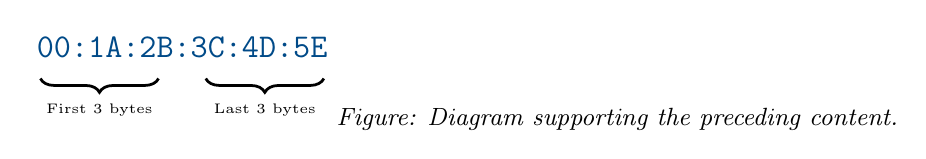
\begin{tikzpicture}
                    % MAC address display
                    \node[font=\large\ttfamily\bfseries, rctcblue] at (0,0) {00:1A:2B:3C:4D:5E};
                    
                    % Breakdown
                    \draw[decorate, decoration={brace, amplitude=5pt, mirror}, line width=1pt]
                        (-1.8,-0.4) -- (-0.3,-0.4);
                    \node[font=\tiny, below] at (-1.05,-0.6) {First 3 bytes};
                    
                    \draw[decorate, decoration={brace, amplitude=5pt, mirror}, line width=1pt]
                        (0.3,-0.4) -- (1.8,-0.4);
                    \node[font=\tiny, below] at (1.05,-0.6) {Last 3 bytes};
                \end{tikzpicture}
            \end{center}
            
            \vspace{0.5em}
            \begin{block}{Common Formats}
                \small
                \texttt{00:1A:2B:3C:4D:5E} (colons) \\
                \texttt{00-1A-2B-3C-4D-5E} (dashes) \\
                \texttt{001A.2B3C.4D5E} (dots---Cisco)
            \end{block}
        \end{column}
    \end{columns}
\end{frame}

% =============================================================================
% SLIDE 11: MAC Address Deep Dive
% =============================================================================
\begin{frame}{MAC Address Deep Dive}
    \begin{columns}[T]
        \begin{column}{0.52\textwidth}
            \begin{itemize}
                \item First 3 bytes: \keyterm{OUI (Organizationally Unique Identifier)}---identifies the manufacturer.
                \item Last 3 bytes: \keyterm{Device ID}---unique to each NIC from that manufacturer.
                \item OUIs are assigned by IEEE---you can look them up online!
            \end{itemize}
            
            \vspace{0.3em}
            \begin{center}
                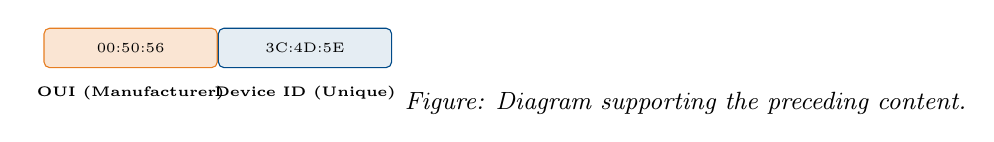
\begin{tikzpicture}
                    \node[frameseg highlight, minimum width=2.2cm] (oui) at (0,0) {00:50:56};
                    \node[frameseg, minimum width=2.2cm, right=0pt of oui] (dev) {3C:4D:5E};
                    
                    \node[font=\tiny\bfseries, below=3pt of oui] {OUI (Manufacturer)};
                    \node[font=\tiny\bfseries, below=3pt of dev] {Device ID (Unique)};
                \end{tikzpicture}
            \end{center}
   
            \begin{exampleblock}{Example OUIs}
                \scriptsize
                \texttt{00:50:56} = VMware \\
                \texttt{00:0C:29} = VMware (alternate) \\
                \texttt{00:1A:A0} = Dell
            \end{exampleblock}
        \end{column}
        \begin{column}{0.45\textwidth}
            \begin{block}{Special MAC Addresses}
                \textbf{Broadcast}: \texttt{FF:FF:FF:FF:FF:FF} \\
                Goes to ALL devices on the network.
                
                \vspace{0.3em}
                \textbf{Multicast}: Starts with \texttt{01:00:5E} \\
                Goes to a group of devices.
            \end{block}
            
            \vspace{0.3em}
            \begin{alertblock}{Can MACs Be Changed?}
                Yes! Software can ``spoof'' a different MAC. Useful for troubleshooting, but also a security concern.
            \end{alertblock}
        \end{column}
    \end{columns}
\end{frame}

% =============================================================================
% SLIDE 12: Case Study - Sam's First NIC Installation
% =============================================================================
\begin{frame}{Case Study: Sam's First NIC Installation}
    \begin{casestudy}{Sam's First NIC Installation}
        Samwise Gamgee is setting up the new admin burrow network for the Shire. He purchases 10 Gbps NICs for the hobbit-hole workstations, but the switches only have SFP ports (1 Gbps, not SFP+).
        
        \vspace{0.5em}
        Sam also notices one workstation showing a MAC address of \texttt{00:00:00:00:00:00} in the network settings.
    \end{casestudy}
    
    \begin{block}{Review Questions}
        \begin{enumerate}
            \item Will the 10 Gbps NICs work in the 1 Gbps switch ports?
            \item What speed will the connection actually operate at?
            \item What might cause a MAC address of all zeros?
        \end{enumerate}
    \end{block}
\end{frame}

% =============================================================================
% SLIDE 13: Case Study Solution - Sam's First NIC Installation
% =============================================================================
\begin{frame}{Case Study Solution: Sam's First NIC Installation}
    \begin{casesolution}{Sam's First NIC Installation}
        \begin{enumerate}
            \item \textbf{Yes}---10 Gbps NICs will auto-negotiate down to match the switch's 1 Gbps capability.
            \item The connection will operate at \textbf{1 Gbps}---limited by the slower device (the switch).
            \item All-zeros MAC address typically means:
                \begin{itemize}
                    \item NIC driver not installed or loaded
                    \item NIC hardware failure
                    \item Virtual/unconfigured network adapter
                \end{itemize}
        \end{enumerate}
    \end{casesolution}
    
    \vspace{0.3em}
    \begin{alertblock}{Key Lessons}
        \begin{itemize}
            \item Always match NIC and switch capabilities for best performance---Sam could save money using 1G NICs.
            \item A missing or abnormal MAC address points to driver or hardware problems.
        \end{itemize}
    \end{alertblock}
\end{frame}

% =============================================================================
% SLIDE 14: The Evolution - Why Switches?
% =============================================================================
\section{Switching Concepts and Forwarding}
\subsection{Hubs, Bridges, and Switches}

\articleonly{
This section compares hub-, bridge-, and switch-based forwarding and explains how modern switches learn and forward traffic efficiently.
}

\begin{frame}{The Evolution: Why Switches?}
    \begin{columns}[T]
        \begin{column}{0.55\textwidth}
            \begin{itemize}
                \item Early networks used \keyterm{hubs}---cheap but problematic.
                \item Then came \keyterm{bridges}---smarter, but limited ports.
                \item Now we use \keyterm{switches}---best of both worlds.
                \item Understanding this evolution helps you troubleshoot legacy networks.
            \end{itemize}
            
            \vspace{0.3em}
            \begin{block}{The Core Problem}
                How do we connect multiple devices efficiently without wasting bandwidth or causing collisions?
            \end{block}
        \end{column}
        \begin{column}{0.42\textwidth}
            \begin{center}
                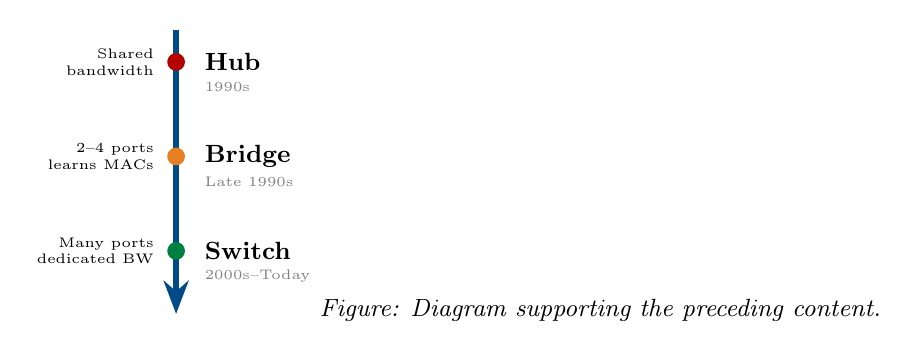
\begin{tikzpicture}[scale=0.8]
                    % Timeline
                    \draw[-{Stealth}, line width=2pt, rctcblue] (0,0) -- (0,-4.5);
                    
                    % Hub
                    \fill[alertred] (0,-0.5) circle (4pt);
                    \node[right, font=\small\bfseries] at (0.3,-0.5) {Hub};
                    \node[right, font=\tiny, gray] at (0.3,-0.9) {1990s};
                    
                    % Bridge
                    \fill[aborange] (0,-2) circle (4pt);
                    \node[right, font=\small\bfseries] at (0.3,-2) {Bridge};
                    \node[right, font=\tiny, gray] at (0.3,-2.4) {Late 1990s};
                    
                    % Switch
                    \fill[networkgreen] (0,-3.5) circle (4pt);
                    \node[right, font=\small\bfseries] at (0.3,-3.5) {Switch};
                    \node[right, font=\tiny, gray] at (0.3,-3.9) {2000s--Today};
                    
                    % Labels
                    \node[left, font=\tiny, align=right] at (-0.2,-0.5) {Shared\\bandwidth};
                    \node[left, font=\tiny, align=right] at (-0.2,-2) {2--4 ports\\learns MACs};
                    \node[left, font=\tiny, align=right] at (-0.2,-3.5) {Many ports\\dedicated BW};
                \end{tikzpicture}
            \end{center}
        \end{column}
    \end{columns}
\end{frame}

% =============================================================================
% SLIDE 15: Hubs - Shared Bandwidth
% =============================================================================
\begin{frame}{Hubs: Shared Bandwidth (and Problems)}
    \begin{columns}[T]
        \begin{column}{0.52\textwidth}
            \begin{itemize}
                \item A \keyterm{hub} repeats every signal to \textbf{every port}.
                \item Like shouting in a room---everyone hears everything.
                \item All devices share the same \keyterm{collision domain}.
                \item Only \textbf{half-duplex} communication possible.
                \item More devices = more collisions = worse performance.
            \end{itemize}
            
            \vspace{0.3em}
            \begin{alertblock}{Why Hubs Are Obsolete}
                10 devices on a 100 Mbps hub = roughly 10 Mbps each (minus collision overhead). Terrible!
            \end{alertblock}
        \end{column}
        \begin{column}{0.45\textwidth}
            \begin{center}
                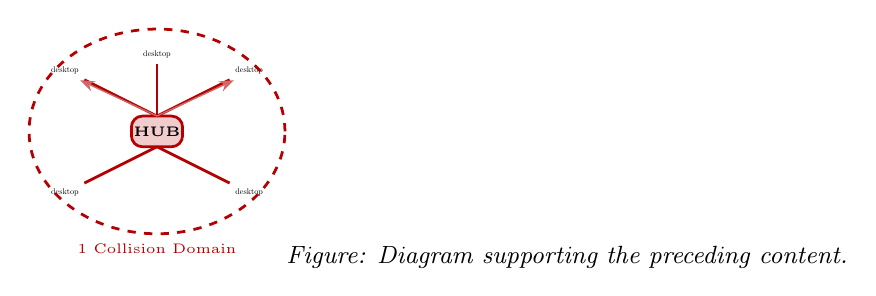
\begin{tikzpicture}[scale=0.65]
                    % Hub
                    \draw[fill=alertred!20, draw=alertred, line width=1pt, rounded corners] 
                        (-0.5,-0.3) rectangle (0.5,0.3);
                    \node[font=\tiny\bfseries] at (0,0) {HUB};
                    
                    % PCs
                    \node[pc] (h1) at (-1.8,1.2) {\iconpc[0.35cm]};
                    \node[pc] (h2) at (0,1.5) {\iconpc[0.35cm]};
                    \node[pc] (h3) at (1.8,1.2) {\iconpc[0.35cm]};
                    \node[pc] (h4) at (-1.8,-1.2) {\iconpc[0.35cm]};
                    \node[pc] (h5) at (1.8,-1.2) {\iconpc[0.35cm]};
                    
                    % Connections
                    \draw[alertred, line width=1pt] (0,0.3) -- (h1);
                    \draw[alertred, line width=1pt] (0,0.3) -- (h2);
                    \draw[alertred, line width=1pt] (0,0.3) -- (h3);
                    \draw[alertred, line width=1pt] (0,-0.3) -- (h4);
                    \draw[alertred, line width=1pt] (0,-0.3) -- (h5);
                    
                    % Collision domain
                    \draw[alertred, dashed, line width=1pt] (0,0) ellipse (2.5cm and 2cm);
                    \node[font=\tiny, alertred] at (0,-2.3) {1 Collision Domain};
                    
                    % Broadcast arrows
                    \draw[-{Stealth}, alertred!60, line width=0.5pt] (0,0.3) -- (-1.5,1);
                    \draw[-{Stealth}, alertred!60, line width=0.5pt] (0,0.3) -- (1.5,1);
                \end{tikzpicture}
            \end{center}
            
            \vspace{0.2em}
            \begin{block}{Hub = Layer 1}
                \small
                Hubs operate at the Physical layer---they don't understand MAC addresses.
            \end{block}
        \end{column}
    \end{columns}
\end{frame}

% =============================================================================
% SLIDE 16: Bridges - Learning MAC Addresses
% =============================================================================
\begin{frame}{Bridges: Learning MAC Addresses}
    \begin{columns}[T]
        \begin{column}{0.52\textwidth}
            \begin{itemize}
                \item A \keyterm{bridge} learns which devices are on which side.
                \item Maintains a \keyterm{MAC address table}.
                \item Only forwards traffic that needs to cross.
                \item Separates \textbf{collision domains}---fewer collisions!
                \item Limited to 2--4 ports (not scalable).
            \end{itemize}
            
            \vspace{0.3em}
            \begin{block}{Bridge = Layer 2}
                Bridges read MAC addresses and make forwarding decisions---smarter than hubs!
            \end{block}
        \end{column}
        \begin{column}{0.45\textwidth}
            \begin{center}
                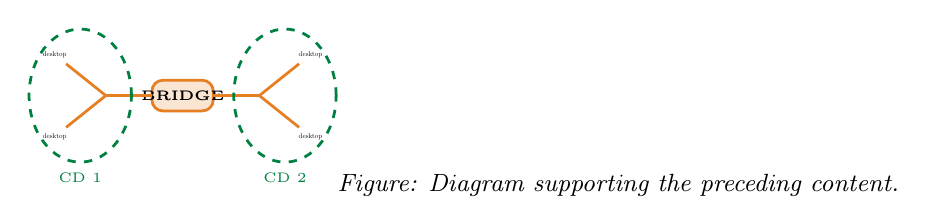
\begin{tikzpicture}[scale=0.65]
                    % Bridge
                    \draw[fill=aborange!20, draw=aborange, line width=1pt, rounded corners] 
                        (-0.6,-0.3) rectangle (0.6,0.3);
                    \node[font=\tiny\bfseries] at (0,0) {BRIDGE};
                    
                    % Left segment
                    \node[pc] (l1) at (-2.5,0.8) {\iconpc[0.3cm]};
                    \node[pc] (l2) at (-2.5,-0.8) {\iconpc[0.3cm]};
                    \draw[aborange, line width=1pt] (-0.6,0) -- (-1.5,0);
                    \draw[aborange, line width=1pt] (-1.5,0) -- (l1);
                    \draw[aborange, line width=1pt] (-1.5,0) -- (l2);
                    
                    % Right segment
                    \node[pc] (r1) at (2.5,0.8) {\iconpc[0.3cm]};
                    \node[pc] (r2) at (2.5,-0.8) {\iconpc[0.3cm]};
                    \draw[aborange, line width=1pt] (0.6,0) -- (1.5,0);
                    \draw[aborange, line width=1pt] (1.5,0) -- (r1);
                    \draw[aborange, line width=1pt] (1.5,0) -- (r2);
                    
                    % Collision domains
                    \draw[networkgreen, dashed, line width=1pt] (-2,0) ellipse (1cm and 1.3cm);
                    \draw[networkgreen, dashed, line width=1pt] (2,0) ellipse (1cm and 1.3cm);
                    
                    % Labels
                    \node[font=\tiny, networkgreen] at (-2,-1.6) {CD 1};
                    \node[font=\tiny, networkgreen] at (2,-1.6) {CD 2};
                \end{tikzpicture}
            \end{center}
            
            \vspace{0.2em}
            \begin{exampleblock}{Selective Forwarding}
                \small
                Traffic between L1 and L2 stays on the left---the bridge doesn't forward it right.
            \end{exampleblock}
        \end{column}
    \end{columns}
\end{frame}

% =============================================================================
% SLIDE 17: Switches - The Modern Solution
% =============================================================================
\begin{frame}{Switches: The Modern Solution}
    \begin{columns}[T]
        \begin{column}{0.52\textwidth}
            \begin{itemize}
                \item A \keyterm{switch} is essentially a multi-port bridge.
                \item Each port is its own \textbf{collision domain}---no collisions!
                \item \textbf{Full-duplex} communication on every port.
                \item \textbf{Dedicated bandwidth} per port (not shared).
                \item Learns MAC addresses automatically.
            \end{itemize}
            
            \vspace{0.3em}
            \begin{exampleblock}{Bandwidth Advantage}
                A 24-port Gigabit switch = up to 24 Gbps total capacity (each port gets full 1 Gbps).
            \end{exampleblock}
        \end{column}
        \begin{column}{0.45\textwidth}
            \begin{center}
                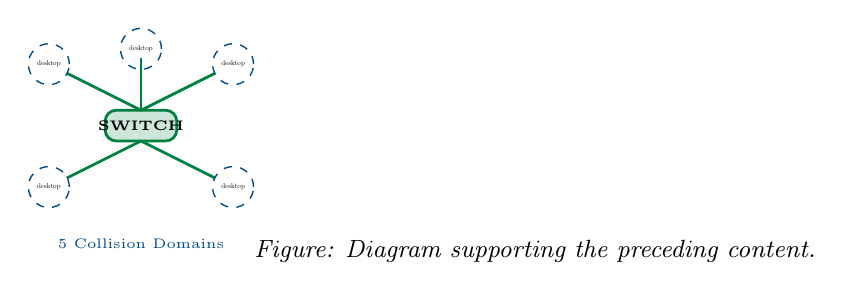
\begin{tikzpicture}[scale=0.65]
                    % Switch
                    \draw[fill=networkgreen!20, draw=networkgreen, line width=1pt, rounded corners] 
                        (-0.7,-0.3) rectangle (0.7,0.3);
                    \node[font=\tiny\bfseries] at (0,0) {SWITCH};
                    
                    % PCs with individual collision domains
                    \node[pc] (s1) at (-1.8,1.2) {\iconpc[0.3cm]};
                    \node[pc] (s2) at (0,1.5) {\iconpc[0.3cm]};
                    \node[pc] (s3) at (1.8,1.2) {\iconpc[0.3cm]};
                    \node[pc] (s4) at (-1.8,-1.2) {\iconpc[0.3cm]};
                    \node[pc] (s5) at (1.8,-1.2) {\iconpc[0.3cm]};
                    
                    % Connections
                    \draw[networkgreen, line width=1pt] (0,0.3) -- (s1);
                    \draw[networkgreen, line width=1pt] (0,0.3) -- (s2);
                    \draw[networkgreen, line width=1pt] (0,0.3) -- (s3);
                    \draw[networkgreen, line width=1pt] (0,-0.3) -- (s4);
                    \draw[networkgreen, line width=1pt] (0,-0.3) -- (s5);
                    
                    % Individual collision domains (small circles)
                    \draw[rctcblue, dashed, line width=0.5pt] (s1) circle (0.4cm);
                    \draw[rctcblue, dashed, line width=0.5pt] (s2) circle (0.4cm);
                    \draw[rctcblue, dashed, line width=0.5pt] (s3) circle (0.4cm);
                    \draw[rctcblue, dashed, line width=0.5pt] (s4) circle (0.4cm);
                    \draw[rctcblue, dashed, line width=0.5pt] (s5) circle (0.4cm);
                    
                    \node[font=\tiny, rctcblue] at (0,-2.3) {5 Collision Domains};
                \end{tikzpicture}
            \end{center}
            
            \vspace{0.2em}
            \begin{block}{Switch = Layer 2}
                \small
                Like bridges, switches read MAC addresses---but with many more ports and better performance.
            \end{block}
        \end{column}
    \end{columns}
\end{frame}

% =============================================================================
% SLIDE 18: How Switches Learn and Forward
% =============================================================================
\begin{frame}{How Switches Learn and Forward}
    \begin{columns}[T]
        \begin{column}{0.48\textwidth}
            \begin{block}{The Four Switch Actions}
                \begin{enumerate}
                    \item \keyterm{Learning}: See source MAC $\rightarrow$ record which port it came from
                    \item \keyterm{Forwarding}: Know destination MAC $\rightarrow$ send only to that port
                    \item \keyterm{Flooding}: Unknown destination $\rightarrow$ send to ALL ports (except source)
                    \item \keyterm{Filtering}: Same-segment traffic $\rightarrow$ don't forward
                \end{enumerate}
            \end{block}
          
        \end{column}
        \begin{column}{0.48\textwidth}
            \begin{center}
                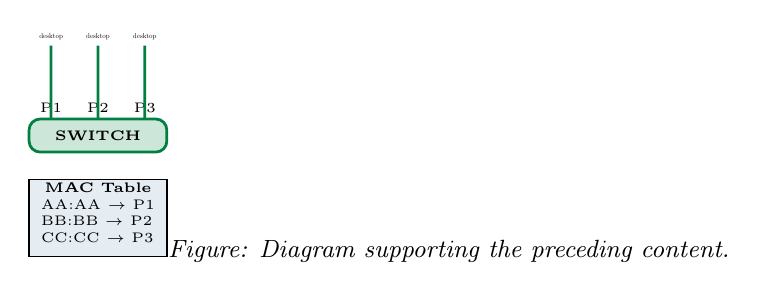
\begin{tikzpicture}[scale=0.7]
                    % Switch
                    \draw[fill=networkgreen!20, draw=networkgreen, line width=1pt, rounded corners] 
                        (0,-0.3) rectangle (2.5,0.3);
                    \node[font=\tiny\bfseries] at (1.25,0) {SWITCH};
                    
                    % Ports labeled
                    \node[font=\tiny] at (0.4,0.5) {P1};
                    \node[font=\tiny] at (1.25,0.5) {P2};
                    \node[font=\tiny] at (2.1,0.5) {P3};
                    
                    % PCs
                    \node[pc] (pc1) at (0.4,1.8) {\iconpc[0.3cm]};
                    \node[pc] (pc2) at (1.25,1.8) {\iconpc[0.3cm]};
                    \node[pc] (pc3) at (2.1,1.8) {\iconpc[0.3cm]};
                    
                    % Connections
                    \draw[networkgreen, line width=1pt] (0.4,0.3) -- (pc1);
                    \draw[networkgreen, line width=1pt] (1.25,0.3) -- (pc2);
                    \draw[networkgreen, line width=1pt] (2.1,0.3) -- (pc3);
                    
                    % MAC table
                    \draw[fill=rctcblue!10, line width=0.5pt] (0,-0.8) rectangle (2.5,-2.2);
                    \node[font=\tiny\bfseries] at (1.25,-0.95) {MAC Table};
                    \node[font=\tiny, align=left] at (1.25,-1.55) {
                        AA:AA $\rightarrow$ P1\\
                        BB:BB $\rightarrow$ P2\\
                        CC:CC $\rightarrow$ P3
                    };
                \end{tikzpicture}
            \end{center}

            \vspace{0.3em}
            \begin{alertblock}{MAC Address Table}
                The switch builds a table mapping MAC addresses to ports. This is how it knows ``who is where.''
            \end{alertblock}

        \end{column}
    \end{columns}
\end{frame}

% =============================================================================
% SLIDE B: Layer 2 Network Diagram - MAC Address Communication
% =============================================================================
\begin{frame}{Layer 2: MAC Address Communication at the Green Dragon}
    \begin{center}
        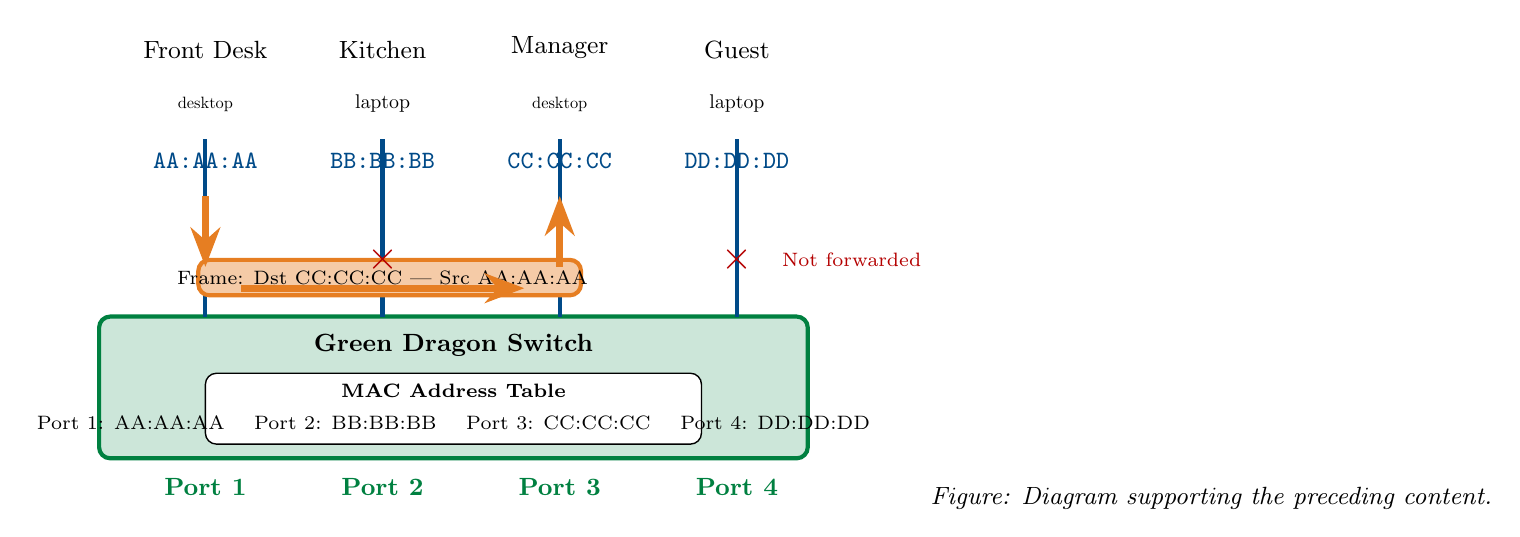
\begin{tikzpicture}[scale=0.9]
            % === SWITCH WITH MAC TABLE ===
            \draw[fill=networkgreen!20, draw=networkgreen, line width=1.5pt, rounded corners] 
                (0,-1) rectangle (10,1);
            \node[font=\small\bfseries] at (5,0.6) {Green Dragon Switch};
            
            % MAC Address Table inside switch
            \draw[fill=white, line width=0.5pt, rounded corners] (1.5,-0.8) rectangle (8.5,0.2);
            \node[font=\scriptsize\bfseries] at (5,-0.05) {MAC Address Table};
            \node[font=\scriptsize] at (5,-0.5) {
                Port 1: AA:AA:AA \quad Port 2: BB:BB:BB \quad Port 3: CC:CC:CC \quad Port 4: DD:DD:DD
            };
            
            % Port labels below switch
            \node[font=\small\bfseries, networkgreen] at (1.5,-1.4) {Port 1};
            \node[font=\small\bfseries, networkgreen] at (4,-1.4) {Port 2};
            \node[font=\small\bfseries, networkgreen] at (6.5,-1.4) {Port 3};
            \node[font=\small\bfseries, networkgreen] at (9,-1.4) {Port 4};
            
            % === DEVICES WITH MAC ADDRESSES ===
            % Front Desk (Port 1)
            \node[pc] (pc1) at (1.5,4) {\iconpc[0.7cm]};
            \node[font=\small, above] at (1.5,4.5) {Front Desk};
            \node[font=\small\ttfamily, rctcblue] at (1.5,3.2) {AA:AA:AA};
            \draw[ethernet noarrow, line width=1.5pt] (1.5,1) -- (1.5,3.5);
            
            % Kitchen (Port 2)
            \node[laptop] (pc2) at (4,4) {\iconlaptop[0.7cm]};
            \node[font=\small, above] at (4,4.5) {Kitchen};
            \node[font=\small\ttfamily, rctcblue] at (4,3.2) {BB:BB:BB};
            \draw[ethernet noarrow, line width=1.5pt] (4,1) -- (4,3.5);
            
            % Manager (Port 3)
            \node[pc] (pc3) at (6.5,4) {\iconpc[0.7cm]};
            \node[font=\small, above] at (6.5,4.5) {Manager};
            \node[font=\small\ttfamily, rctcblue] at (6.5,3.2) {CC:CC:CC};
            \draw[ethernet noarrow, line width=1.5pt] (6.5,1) -- (6.5,3.5);
            
            % Guest (Port 4)
            \node[laptop] (pc4) at (9,4) {\iconlaptop[0.7cm]};
            \node[font=\small, above] at (9,4.5) {Guest};
            \node[font=\small\ttfamily, rctcblue] at (9,3.2) {DD:DD:DD};
            \draw[ethernet noarrow, line width=1.5pt] (9,1) -- (9,3.5);
            
            % === FRAME BEING FORWARDED ===
            % Frame traveling from Front Desk to Manager
            \draw[fill=aborange!40, draw=aborange, line width=1.5pt, rounded corners]
                (1.4,1.3) rectangle (6.8,1.8);
            \node[font=\scriptsize] at (4,1.55) {Frame: Dst CC:CC:CC | Src AA:AA:AA};
            
            % Arrow showing forwarding path - into switch
            \draw[-{Stealth}, aborange, line width=2.5pt] (1.5,2.7) -- (1.5,1.7);
            
            % Arrow through switch
            \draw[-{Stealth}, aborange, line width=2.5pt] (2,1.4) -- (6,1.4);
            
            % Arrow out to Manager
            \draw[-{Stealth}, aborange, line width=2.5pt] (6.5,1.7) -- (6.5,2.7);
            
            % X marks on ports NOT receiving the frame
            \node[font=\Large, alertred] at (4,1.8) {$\times$};
            \node[font=\Large, alertred] at (9,1.8) {$\times$};
            
            % Annotation for blocked ports
            \node[font=\scriptsize, alertred, right] at (9.5,1.8) {Not forwarded};
        \end{tikzpicture}
    \end{center}
    
    \vspace{0.2em}
    {\centering Layer 2 uses \textbf{MAC addresses} to forward frames. The switch sends traffic \textbf{only to the destination port}---not everywhere.\par}
\end{frame}

% =============================================================================
% SLIDE 19: Unmanaged vs Managed Switches
% =============================================================================
\section{Switch Interfaces and Management}
\subsection{Switch Features and Configuration}

\articleonly{
This section focuses on operational switch features and management choices used in real deployments.
}

\begin{frame}{Unmanaged vs Managed Switches}
    \begin{columns}[T]
        \begin{column}{0.48\textwidth}
            \begin{block}{Unmanaged Switch}
                \begin{itemize}
                    \item Plug and play---no configuration
                    \item No VLANs, no monitoring
                    \item Cheapest option
                    \item Best for: Home, very small office
                \end{itemize}
            \end{block}
            
            \vspace{0.3em}
            \begin{block}{Smart Switch}
                \begin{itemize}
                    \item Some management features
                    \item Basic VLANs, simple web GUI
                    \item Middle price range
                    \item Best for: Small business
                \end{itemize}
            \end{block}
        \end{column}
        \begin{column}{0.48\textwidth}
            \begin{block}{Managed Switch}
                \begin{itemize}
                    \item Full configuration options
                    \item VLANs, STP, SNMP, port security
                    \item CLI, web GUI, remote management
                    \item Best for: Enterprise networks
                \end{itemize}
            \end{block}
            
            \vspace{0.3em}
            \begin{exampleblock}{Key Question}
                Do you need to separate traffic, monitor performance, or configure security? If yes $\rightarrow$ managed switch.
            \end{exampleblock}
        \end{column}
    \end{columns}
\end{frame}

% =============================================================================
% SLIDE 20: Layer 2 vs Layer 3 Switches
% =============================================================================
\begin{frame}{Layer 2 vs Layer 3 Switches}
    \begin{columns}[T]
        \begin{column}{0.48\textwidth}
            \begin{block}{Layer 2 Switch (Standard)}
                \begin{itemize}
                    \item Forwards based on \textbf{MAC addresses}
                    \item Cannot route between networks
                    \item Needs a router for inter-VLAN traffic
                    \item Less expensive
                \end{itemize}
                
                \centering
                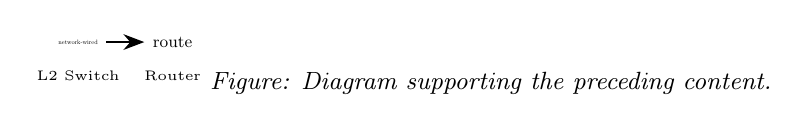
\begin{tikzpicture}[scale=0.6]
                    \node[font=\small] at (0,0) {\iconswitch[0.5cm]};
                    \node[font=\tiny, below] at (0,-0.4) {L2 Switch};
                    \draw[-{Stealth}, line width=1pt] (0.6,0) -- (1.4,0);
                    \node[font=\small] at (2,0) {\iconrouter[0.5cm]};
                    \node[font=\tiny, below] at (2,-0.4) {Router};
                \end{tikzpicture}
            \end{block}
        \end{column}
        \begin{column}{0.48\textwidth}
            \begin{block}{Layer 3 Switch (Multilayer)}
                \begin{itemize}
                    \item Also routes based on \textbf{IP addresses}
                    \item Can route between VLANs directly
                    \item Faster than using separate router
                    \item More expensive
                \end{itemize}
                
                \centering
                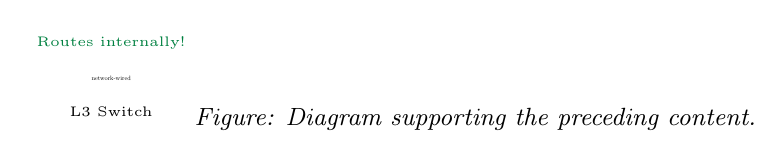
\begin{tikzpicture}[scale=0.6]
                    \node[font=\small] at (0,0) {\iconswitch[0.5cm]};
                    \node[font=\tiny, below] at (0,-0.4) {L3 Switch};
                    \node[font=\tiny, above, networkgreen] at (0,0.4) {Routes internally!};
                \end{tikzpicture}
            \end{block}
        \end{column}
    \end{columns}
    
    \vspace{0.3em}
    \begin{alertblock}{When to Use Layer 3 Switches}
        Large networks with multiple VLANs benefit from Layer 3 switches---inter-VLAN traffic stays fast without bottlenecking through a router.
    \end{alertblock}
\end{frame}

% =============================================================================
% SLIDE 21: Switch Interface Configuration Basics
% =============================================================================
\begin{frame}{Switch Interface Configuration Basics}
    \begin{columns}[T]
        \begin{column}{0.48\textwidth}
            \begin{block}{Access Methods}
                \begin{itemize}
                    \item \keyterm{Console cable}: Direct serial connection (initial setup)
                    \item \keyterm{SSH/Telnet}: Remote CLI over network
                    \item \keyterm{Web GUI}: Browser-based (some models)
                \end{itemize}
            \end{block}
            
            \vspace{0.3em}
            \begin{block}{Common Settings}
                \begin{itemize}
                    \item Port speed (10/100/1000)
                    \item Duplex mode (half/full/auto)
                    \item VLAN assignment
                    \item Port description/label
                \end{itemize}
            \end{block}
        \end{column}
        \begin{column}{0.48\textwidth}
            \begin{alertblock}{Speed/Duplex Mismatch}
                If one side is set to auto and the other is manually configured, they may negotiate incorrectly. Result: slow speeds, errors, packet loss.
            \end{alertblock}
            
            \vspace{0.3em}
            \begin{exampleblock}{Port Security}
                Limit which MAC addresses can connect to a port:
                \begin{itemize}
                    \item Prevent unauthorized devices
                    \item Protect against MAC flooding attacks
                    \item Can shut down port on violation
                \end{itemize}
            \end{exampleblock}
        \end{column}
    \end{columns}
\end{frame}

% =============================================================================
% SLIDE 22: Case Study - The Green Dragon Inn Network
% =============================================================================
\begin{frame}{Case Study: The Green Dragon Inn Network}
    \begin{casestudy}{The Green Dragon Inn Network}
        The Green Dragon Inn is expanding and needs a network for guest hobbits and staff. Frodo suggests a cheap unmanaged switch. Gandalf recommends a managed switch instead.
        
        \vspace{0.5em}
        The network requirements:
        \begin{itemize}
            \item Separate guest traffic from staff traffic (security)
            \item Support 20 devices total
            \item Allow remote management (Gandalf travels frequently)
        \end{itemize}
    \end{casestudy}
    
    \begin{block}{Review Questions}
        \begin{enumerate}
            \item Which switch type should they choose and why?
            \item What feature would separate guest from staff traffic?
            \item Why is remote management valuable for an inn?
        \end{enumerate}
    \end{block}
\end{frame}

% =============================================================================
% SLIDE 23: Case Study Solution - The Green Dragon Inn Network
% =============================================================================
\begin{frame}{Case Study Solution: The Green Dragon Inn Network}
    \begin{casesolution}{The Green Dragon Inn Network}
        \begin{enumerate}
            \item \textbf{Managed switch}---unmanaged switches cannot separate traffic or be configured remotely.
            \item \keyterm{VLANs (Virtual LANs)} separate guest and staff traffic logically on the same physical switch.
            \item Remote management benefits:
                \begin{itemize}
                    \item Gandalf can troubleshoot from anywhere in Middle-earth
                    \item Monitor bandwidth usage and detect problems
                    \item Make changes without disrupting inn operations
                \end{itemize}
        \end{enumerate}
    \end{casesolution}
    
    \vspace{0.3em}
    \begin{alertblock}{Key Lesson}
        The extra cost of managed switches pays off in flexibility and security. For any business network, managed is the right choice.
    \end{alertblock}
\end{frame}

% =============================================================================
% SLIDE 24: Link Aggregation and NIC Teaming
% =============================================================================
\section{Advanced Switching Topics}
\subsection{Resiliency and Performance Features}

\articleonly{
Advanced switching capabilities improve resiliency, bandwidth utilization, and loop prevention in larger networks.
}

\begin{frame}{Link Aggregation and NIC Teaming}
    \begin{columns}[T]
        \begin{column}{0.52\textwidth}
            \begin{itemize}
                \item Problem: One cable isn't fast enough for a busy server.
                \item Solution: Bundle multiple cables together!
                \item \keyterm{Link Aggregation (LAG)}: Combines switch ports into one logical link.
                \item \keyterm{LACP (802.3ad)}: Protocol that negotiates aggregation automatically.
                \item \keyterm{NIC Teaming}: Same concept on the server side.
            \end{itemize}
            
            \vspace{0.3em}
            \begin{block}{Benefits}
                \textbf{More bandwidth}: 4 × 1G = 4 Gbps total \\
                \textbf{Redundancy}: If one link fails, others continue
            \end{block}
        \end{column}
        \begin{column}{0.45\textwidth}
            \begin{center}
                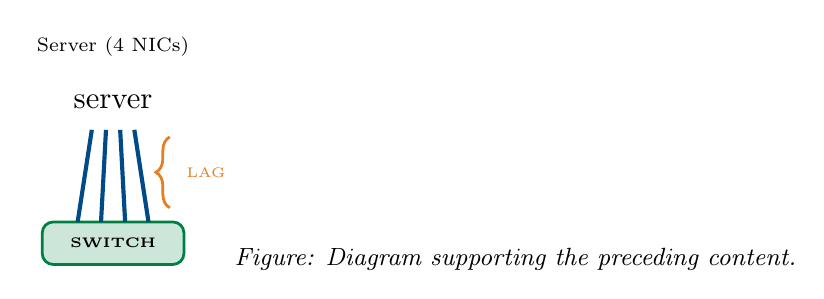
\begin{tikzpicture}[scale=0.9]
                    % Server
                    \node[server] (srv) at (0,2) {\iconserver[1cm]};
                    \node[font=\scriptsize, above] at (0,2.5) {Server (4 NICs)};
                    
                    % Switch
                    \draw[fill=networkgreen!20, draw=networkgreen, line width=1pt, rounded corners] 
                        (-1,-0.3) rectangle (1,0.3);
                    \node[font=\tiny\bfseries] at (0,0) {SWITCH};
                    
                    % Multiple links
                    \draw[rctcblue, line width=1.5pt] (-0.5,0.3) -- (-0.3,1.6);
                    \draw[rctcblue, line width=1.5pt] (-0.17,0.3) -- (-0.1,1.6);
                    \draw[rctcblue, line width=1.5pt] (0.17,0.3) -- (0.1,1.6);
                    \draw[rctcblue, line width=1.5pt] (0.5,0.3) -- (0.3,1.6);
                    
                    % LAG bracket
                    \draw[decorate, decoration={brace, amplitude=5pt}, line width=1pt, aborange]
                        (0.8,0.5) -- (0.8,1.5);
                    \node[font=\tiny, right, aborange] at (0.9,1) {LAG};
                \end{tikzpicture}
            \end{center}
            
            \vspace{0.3em}
            \begin{alertblock}{Both Ends Must Match}
                LAG must be configured on both the switch AND the server/other switch.
            \end{alertblock}
        \end{column}
    \end{columns}
\end{frame}

% =============================================================================
% SLIDE 25: Maximum Transmission Unit (MTU)
% =============================================================================
\begin{frame}{Maximum Transmission Unit (MTU)}
    \begin{columns}[T]
        \begin{column}{0.52\textwidth}
            \begin{itemize}
                \item \keyterm{MTU}: Maximum frame payload size a network can handle.
                \item Standard Ethernet MTU: \textbf{1500 bytes}.
                \item \keyterm{Jumbo frames}: MTU up to \textbf{9000 bytes}---more efficient for large transfers.
                \item Larger frames = fewer frames = less overhead.
            \end{itemize}
            
            \vspace{0.3em}
            \begin{alertblock}{Critical Requirement}
                \textbf{Every device in the path} must support the same MTU! Mismatched MTU causes fragmentation or dropped packets.
            \end{alertblock}
        \end{column}
        \begin{column}{0.45\textwidth}
            \begin{center}
                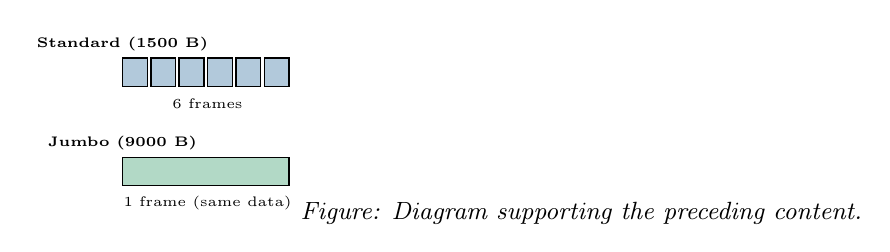
\begin{tikzpicture}[scale=0.9]
                    % Standard frame
                    \node[font=\tiny\bfseries] at (0,1.8) {Standard (1500 B)};
                    \foreach \x in {0,0.4,0.8,1.2,1.6,2.0} {
                        \draw[fill=rctcblue!30, line width=0.5pt] (\x,1.2) rectangle (\x+0.35,1.6);
                    }
                    \node[font=\tiny] at (1.2,0.95) {6 frames};
                    
                    % Jumbo frame
                    \node[font=\tiny\bfseries] at (0,0.4) {Jumbo (9000 B)};
                    \draw[fill=networkgreen!30, line width=0.5pt] (0,-0.2) rectangle (2.35,0.2);
                    \node[font=\tiny] at (1.2,-0.45) {1 frame (same data)};
                \end{tikzpicture}
            \end{center}
            
            \vspace{0.3em}
            \begin{block}{When to Use Jumbo Frames}
                \begin{itemize}
                    \item Storage networks (iSCSI, NFS)
                    \item Backup systems
                    \item Data center internal traffic
                \end{itemize}
            \end{block}
        \end{column}
    \end{columns}
\end{frame}

% =============================================================================
% SLIDE 26: Spanning Tree Protocol - The Problem
% =============================================================================
\begin{frame}{Spanning Tree Protocol: The Problem}
    \begin{columns}[T]
        \begin{column}{0.52\textwidth}
            \begin{itemize}
                \item What happens if you create a \keyterm{loop} in a switched network?
                \item Frames have no TTL (time-to-live) at Layer 2---they circulate forever!
                \item Result: \keyterm{Broadcast storm}---frames multiply exponentially.
                \item Network grinds to a halt in seconds.
                \item Loops happen accidentally (wrong cable) or intentionally (redundancy gone wrong).
            \end{itemize}
            
            \vspace{0.3em}
            \begin{alertblock}{Real Danger}
                An accidental loop can crash an entire network in under 30 seconds!
            \end{alertblock}
        \end{column}
        \begin{column}{0.45\textwidth}
            \begin{center}
                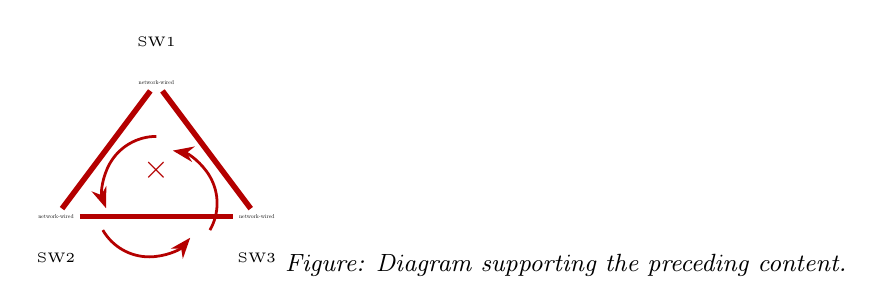
\begin{tikzpicture}[scale=0.85]
                    % Three switches in triangle
                    \node[switch] (sw1) at (0,2) {\iconswitch[0.45cm]};
                    \node[switch] (sw2) at (-1.5,0) {\iconswitch[0.45cm]};
                    \node[switch] (sw3) at (1.5,0) {\iconswitch[0.45cm]};
                    
                    % Labels
                    \node[font=\tiny, above] at (0,2.4) {SW1};
                    \node[font=\tiny, below] at (-1.5,-0.4) {SW2};
                    \node[font=\tiny, below] at (1.5,-0.4) {SW3};
                    
                    % Connections forming loop
                    \draw[alertred, line width=2pt] (sw1) -- (sw2);
                    \draw[alertred, line width=2pt] (sw2) -- (sw3);
                    \draw[alertred, line width=2pt] (sw3) -- (sw1);
                    
                    % Circular arrows showing loop
                    \draw[-{Stealth}, alertred, line width=1pt] 
                        (0,1.2) arc (90:200:0.8);
                    \draw[-{Stealth}, alertred, line width=1pt] 
                        (-0.8,-0.2) arc (210:320:0.8);
                    \draw[-{Stealth}, alertred, line width=1pt] 
                        (0.8,-0.2) arc (-30:80:0.8);
                    
                    % Explosion symbol
                    \node[font=\large, alertred] at (0,0.7) {$\times$};
                \end{tikzpicture}
            \end{center}
            
            \vspace{0.3em}
            \begin{block}{Symptoms}
                \small
                All switch LEDs flashing rapidly, network unresponsive, high CPU on switches.
            \end{block}
        \end{column}
    \end{columns}
\end{frame}

% =============================================================================
% SLIDE 27: Spanning Tree Protocol - The Solution
% =============================================================================
\begin{frame}{Spanning Tree Protocol: The Solution}
    \begin{columns}[T]
        \begin{column}{0.52\textwidth}
            \begin{itemize}
                \item \keyterm{STP (802.1D)} automatically detects and blocks redundant paths.
                \item Elects a \keyterm{root bridge}---the central reference point.
                \item Calculates best path from each switch to the root.
                \item \keyterm{Blocks} redundant ports to prevent loops.
                \item If active link fails, blocked port activates---redundancy preserved!
            \end{itemize}
            
            \vspace{0.3em}
            \begin{block}{STP Versions}
                \small
                \textbf{802.1D (STP)}: Original, slow (30--50 sec) \\
                \textbf{802.1w (RSTP)}: Rapid, fast (1--2 sec) \\
                \textbf{802.1s (MSTP)}: Per-VLAN spanning trees
            \end{block}
        \end{column}
        \begin{column}{0.45\textwidth}
            \begin{center}
                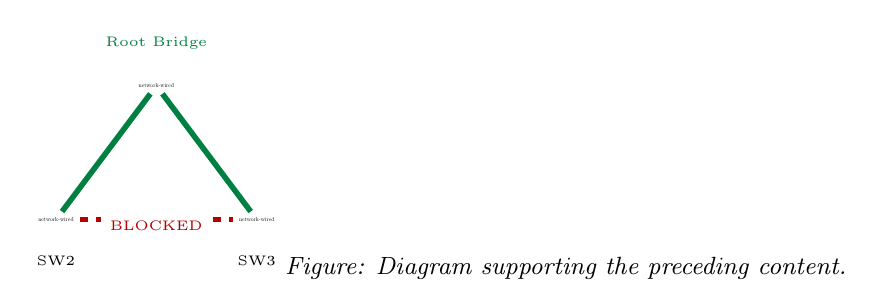
\begin{tikzpicture}[scale=0.85]
                    % Three switches in triangle
                    \node[switch] (sw1) at (0,2) {\iconswitch[0.45cm]};
                    \node[switch] (sw2) at (-1.5,0) {\iconswitch[0.45cm]};
                    \node[switch] (sw3) at (1.5,0) {\iconswitch[0.45cm]};
                    
                    % Labels
                    \node[font=\tiny, above, networkgreen] at (0,2.4) {Root Bridge};
                    \node[font=\tiny, below] at (-1.5,-0.4) {SW2};
                    \node[font=\tiny, below] at (1.5,-0.4) {SW3};
                    
                    % Active connections (green)
                    \draw[networkgreen, line width=2pt] (sw1) -- (sw2);
                    \draw[networkgreen, line width=2pt] (sw1) -- (sw3);
                    
                    % Blocked connection (dashed red)
                    \draw[alertred, line width=2pt, dashed] (sw2) -- (sw3);
                    
                    % Blocked symbol
                    \node[font=\tiny, alertred, fill=white] at (0,-0.1) {BLOCKED};
                \end{tikzpicture}
            \end{center}
            
            \vspace{0.3em}
            \begin{exampleblock}{Key Insight}
                STP provides redundancy WITHOUT loops---blocked ports wait as backups.
            \end{exampleblock}
        \end{column}
    \end{columns}
\end{frame}

% =============================================================================
% SLIDE 28: Power over Ethernet (PoE)
% =============================================================================
\begin{frame}{Power over Ethernet (PoE)}
    \begin{columns}[T]
        \begin{column}{0.52\textwidth}
            \begin{itemize}
                \item \keyterm{PoE} delivers electrical power AND data over the same Ethernet cable.
                \item No separate power outlet needed at the device!
                \item Perfect for: IP phones, security cameras, wireless access points, IoT devices.
                \item Switch must be \keyterm{PoE-capable} or use a separate \keyterm{PoE injector}.
            \end{itemize}
            
            \vspace{0.3em}
            \begin{alertblock}{Power Budget}
                Switches have a total PoE power budget (e.g., 370W). Plan carefully---you can't power unlimited devices!
            \end{alertblock}
        \end{column}
        \begin{column}{0.45\textwidth}
            \begin{center}
                \scriptsize
                \begin{tabular}{l c l}
                    \toprule
                    \textbf{Standard} & \textbf{Power} & \textbf{Devices} \\
                    \midrule
                    802.3af & 15.4W & IP phones \\
                    802.3at (PoE+) & 30W & Cameras, APs \\
                    802.3bt (PoE++) & 60--100W & PTZ cameras \\
                    \bottomrule
                \end{tabular}
            \end{center}
            
            \vspace{0.5em}
            \begin{block}{PoE Advantage}
                \centering
                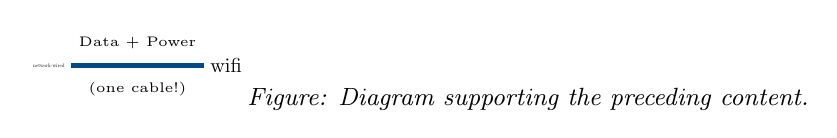
\begin{tikzpicture}[scale=0.9]
                    % Switch
                    \node[switch] (sw) at (0,0) {\iconswitch[0.4cm]};
                    
                    % AP
                    \node[wifi] (ap) at (2.5,0) {\iconwifi[0.4cm]};
                    
                    % Single cable
                    \draw[rctcblue, line width=1.5pt] (sw) -- (ap);
                    
                    % Labels
                    \node[font=\tiny, above] at (1.25,0.1) {Data + Power};
                    \node[font=\tiny, below] at (1.25,-0.1) {(one cable!)};
                \end{tikzpicture}
            \end{block}
        \end{column}
    \end{columns}
\end{frame}

% =============================================================================
% SLIDE C: PoE Network Diagram - Power Budget at the Green Dragon
% =============================================================================
\begin{frame}{Power over Ethernet: Green Dragon Power Budget}
    \begin{center}
        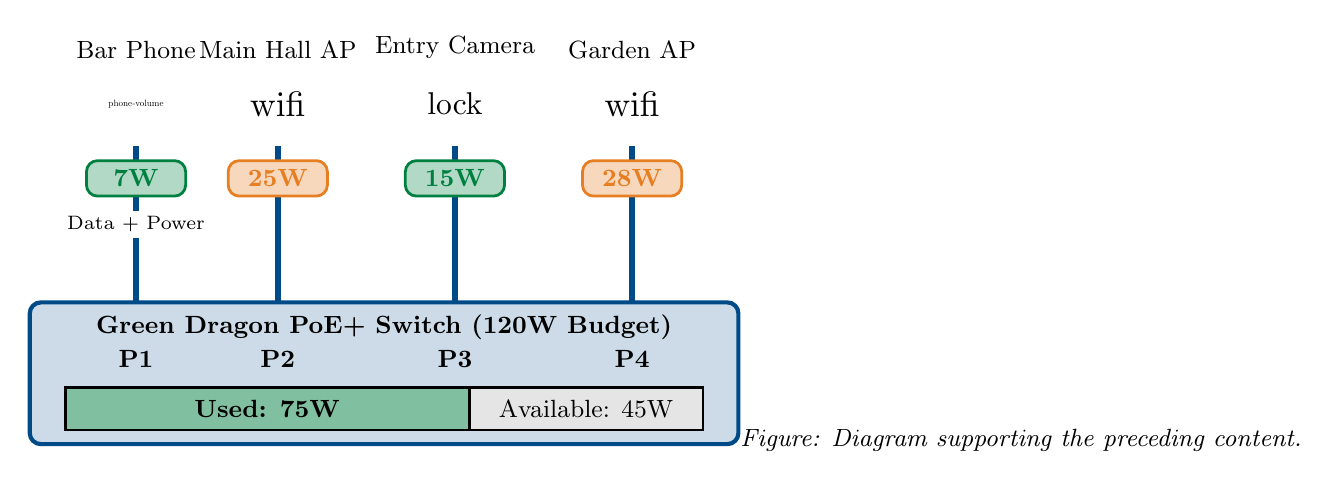
\begin{tikzpicture}[scale=0.9]
            % === POE SWITCH ===
            \draw[fill=rctcblue!20, draw=rctcblue, line width=1.5pt, rounded corners] 
                (0,-1.3) rectangle (10,0.7);
            \node[font=\small\bfseries] at (5,0.35) {Green Dragon PoE+ Switch (120W Budget)};
            
            % Power budget bar
            \draw[fill=gray!20, line width=1pt] (0.5,-1.1) rectangle (9.5,-0.5);
            % Used power section (75W out of 120W = 62.5%)
            \draw[fill=networkgreen!50, line width=1pt] (0.5,-1.1) rectangle (6.2,-0.5);
            \node[font=\small\bfseries] at (3.35,-0.8) {Used: 75W};
            \node[font=\small] at (7.85,-0.8) {Available: 45W};
            
            % Port indicators on switch
            \node[font=\small\bfseries] at (1.5,-0.1) {P1};
            \node[font=\small\bfseries] at (3.5,-0.1) {P2};
            \node[font=\small\bfseries] at (6,-0.1) {P3};
            \node[font=\small\bfseries] at (8.5,-0.1) {P4};
            
            % === POE DEVICES ===
            
            % VoIP Phone (P1) - 7W
            \node[phone] (phone) at (1.5,3.5) {\iconvoip[0.7cm]};
            \node[font=\small, above] at (1.5,4) {Bar Phone};
            \draw[rctcblue, line width=2pt] (1.5,0.7) -- (1.5,2.9);
            \node[font=\scriptsize, fill=white, inner sep=2pt] at (1.5,1.8) {Data + Power};
            % Power box
            \draw[fill=networkgreen!30, draw=networkgreen, line width=1pt, rounded corners]
                (0.8,2.2) rectangle (2.2,2.7);
            \node[font=\small\bfseries, networkgreen] at (1.5,2.45) {7W};
            
            % Wireless AP (P2) - 25W
            \node[wifi] (ap) at (3.5,3.5) {\iconwifi[0.7cm]};
            \node[font=\small, above] at (3.5,4) {Main Hall AP};
            \draw[rctcblue, line width=2pt] (3.5,0.7) -- (3.5,2.9);
            % Power box
            \draw[fill=aborange!30, draw=aborange, line width=1pt, rounded corners]
                (2.8,2.2) rectangle (4.2,2.7);
            \node[font=\small\bfseries, aborange] at (3.5,2.45) {25W};
            
            % Security Camera (P3) - 15W
            \node (cam) at (6,3.5) {\iconlock[0.7cm]};
            \node[font=\small, above] at (6,4) {Entry Camera};
            \draw[rctcblue, line width=2pt] (6,0.7) -- (6,2.9);
            % Power box
            \draw[fill=networkgreen!30, draw=networkgreen, line width=1pt, rounded corners]
                (5.3,2.2) rectangle (6.7,2.7);
            \node[font=\small\bfseries, networkgreen] at (6,2.45) {15W};
            
            % Second AP (P4) - 28W
            \node[wifi] (ap2) at (8.5,3.5) {\iconwifi[0.7cm]};
            \node[font=\small, above] at (8.5,4) {Garden AP};
            \draw[rctcblue, line width=2pt] (8.5,0.7) -- (8.5,2.9);
            % Power box
            \draw[fill=aborange!30, draw=aborange, line width=1pt, rounded corners]
                (7.8,2.2) rectangle (9.2,2.7);
            \node[font=\small\bfseries, aborange] at (8.5,2.45) {28W};
            
           
        \end{tikzpicture}
    \end{center}
    
    \vspace{0.1em}
    {\centering PoE delivers \textbf{data and power} over one cable. Always track your \textbf{power budget}---the switch has limits!\par}
\end{frame}

% =============================================================================
% SLIDE 29: Case Study - Bilbo's Birthday Party Network Disaster
% =============================================================================
\begin{frame}{Case Study: Bilbo's Birthday Party Network Disaster}
    \begin{casestudy}{Bilbo's Birthday Party Network Disaster}
        Bilbo is hosting his 111th birthday party and needs a network for the event planners. Shortly after setup, the entire network crashes---all switches show frantically blinking lights, and no device can communicate.
        
        \vspace{0.5em}
        Merry investigates and discovers someone connected both ends of a patch cable to the same switch to ``make the cables neater.''
    \end{casestudy}
    
    \begin{block}{Review Questions}
        \begin{enumerate}
            \item What has happened to the network?
            \item What protocol should have prevented this?
            \item What should they check on the switches?
        \end{enumerate}
    \end{block}
\end{frame}

% =============================================================================
% SLIDE 30: Case Study Solution - Bilbo's Birthday Party Network Disaster
% =============================================================================
\begin{frame}{Case Study Solution: Bilbo's Birthday Party Network Disaster}
    \begin{casesolution}{Bilbo's Birthday Party Network Disaster}
        \begin{enumerate}
            \item A \keyterm{switching loop} caused a \keyterm{broadcast storm}---frames multiplied until they overwhelmed every switch.
            \item \keyterm{Spanning Tree Protocol (STP)} should block redundant paths automatically.
            \item Immediate actions:
                \begin{itemize}
                    \item Remove the looped cable immediately
                    \item Check if STP is enabled on all switches
                    \item Verify switches are managed (unmanaged switches may lack STP)
                \end{itemize}
        \end{enumerate}
    \end{casesolution}
    
    \vspace{0.3em}
    \begin{alertblock}{Key Lesson}
        Always use managed switches with STP enabled for any business network. A single accidental loop can take down everything!
    \end{alertblock}
\end{frame}

% =============================================================================
% SLIDE 31: Hardware Failure and Port Status Indicators
% =============================================================================
\section{Troubleshooting Interfaces and Switches}
\subsection{Operational Diagnostics}

\articleonly{
The final section applies structured troubleshooting to interface and switch faults using indicators, commands, and counter analysis.
}

\begin{frame}{Hardware Failure and Port Status Indicators}
    \begin{columns}[T]
        \begin{column}{0.48\textwidth}
            \begin{block}{LED Indicators}
                \begin{itemize}
                    \item \textcolor{networkgreen}{\textbf{Solid green}}: Link up, connected
                    \item \textcolor{networkgreen}{\textbf{Flashing green}}: Active traffic
                    \item \textcolor{aborange}{\textbf{Amber/Orange}}: Error or disabled
                    \item \textbf{Off}: No link detected
                \end{itemize}
            \end{block}
            
            \vspace{0.3em}
            \begin{alertblock}{First Troubleshooting Step}
                Always look at the lights! LEDs tell you port status instantly without logging in.
            \end{alertblock}
        \end{column}
        \begin{column}{0.48\textwidth}
            \begin{block}{Common Hardware Failures}
                \begin{itemize}
                    \item Bad switch port (try another port)
                    \item Failed transceiver module
                    \item Power supply issues
                    \item Overheating (check fans, vents)
                    \item Failed backplane (multiple ports down)
                \end{itemize}
            \end{block}
            
            \vspace{0.3em}
            \begin{exampleblock}{No Link Light?}
                Check in order: cable $\rightarrow$ NIC $\rightarrow$ switch port $\rightarrow$ transceiver (if applicable).
            \end{exampleblock}
        \end{column}
    \end{columns}
\end{frame}

% =============================================================================
% SLIDE 32: Switch Show Commands
% =============================================================================
\begin{frame}{Switch Show Commands}
    \begin{columns}[T]
        \begin{column}{0.48\textwidth}
            \begin{block}{Essential Commands}
                \small
                \texttt{\textbf{show interfaces}} \\
                Port status, speed, duplex, errors
                
                \vspace{0.3em}
                \texttt{\textbf{show mac address-table}} \\
                Which MACs learned on which ports
                
                \vspace{0.3em}
                \texttt{\textbf{show spanning-tree}} \\
                STP status, root bridge, blocked ports
                
                \vspace{0.3em}
                \texttt{\textbf{show power inline}} \\
                PoE status and power consumption
            \end{block}
        \end{column}
        \begin{column}{0.48\textwidth}
            \begin{block}{Example Output}
                \ttfamily\scriptsize
                Switch\# show interfaces Gi0/1 \\
                GigabitEthernet0/1 is up \\
                \ \ Speed: 1000 Mbps, Duplex: Full \\
                \ \ Input errors: 0, CRC: 0 \\
                \ \ Output errors: 0, Collisions: 0
            \end{block}
            
            \vspace{0.3em}
            \begin{alertblock}{Key Insight}
                These commands work on Cisco and many other managed switches. Learn them once, use them everywhere.
            \end{alertblock}
        \end{column}
    \end{columns}
\end{frame}

% =============================================================================
% SLIDE 33: Interface Error Counters
% =============================================================================
\begin{frame}{Interface Error Counters}
    \begin{columns}[T]
        \begin{column}{0.48\textwidth}
            \begin{block}{Error Types}
                \keyterm{CRC errors}: Damaged frames---bad cable, NIC, or interference.
                
                \vspace{0.3em}
                \keyterm{Collisions}: Duplex mismatch or hub in path.
                
                \vspace{0.3em}
                \keyterm{Runts}: Frames too small ($<$64 bytes)---collision fragments.
                
                \vspace{0.3em}
                \keyterm{Giants}: Frames too large---MTU mismatch.
            \end{block}
        \end{column}
        \begin{column}{0.48\textwidth}
            \begin{block}{Input/Output Errors}
                \keyterm{Input errors}: Problems receiving frames.
                
                \vspace{0.3em}
                \keyterm{Output errors}: Problems sending frames.
                
                \vspace{0.3em}
                \keyterm{Discards}: Frames dropped (buffer full, policy).
            \end{block}
            
            \vspace{0.3em}
            \begin{alertblock}{Interpretation}
                A few errors = normal. \\
                Rapidly increasing = active problem!
            \end{alertblock}
        \end{column}
    \end{columns}
    
    \vspace{0.3em}
    \begin{exampleblock}{Pro Tip}
        Clear counters, wait 5 minutes, check again. If errors accumulate quickly, investigate that port.
    \end{exampleblock}
\end{frame}

% =============================================================================
% SLIDE 34: MAC Address Table Troubleshooting
% =============================================================================
\begin{frame}{MAC Address Table Troubleshooting}
    \begin{columns}[T]
        \begin{column}{0.48\textwidth}
            \begin{itemize}
                \item The \keyterm{MAC address table} shows which devices the switch has learned.
                \item Use it to verify: Is the device connected? Which port?
                \item If a MAC appears on the wrong port---cable may be in wrong jack.
                \item If a MAC is missing---device may be off, disconnected, or NIC failed.
            \end{itemize}
            
            \vspace{0.3em}
            \begin{block}{Command}
                \texttt{show mac address-table}
            \end{block}
        \end{column}
        \begin{column}{0.48\textwidth}
            \begin{block}{Example Output}
                \ttfamily\scriptsize
                VLAN \ \ MAC Address \ \ \ \ \ Port \\
                ---- \ \ ----------- \ \ \ \ \ ---- \\
                1 \ \ \ \ 00:1A:2B:3C:4D:5E \ Gi0/1 \\
                1 \ \ \ \ 00:50:56:AA:BB:CC \ Gi0/2 \\
                1 \ \ \ \ FF:FF:FF:FF:FF:FF \ CPU
            \end{block}
            
            \vspace{0.3em}
            \begin{alertblock}{MAC Flapping}
                Same MAC appearing on multiple ports rapidly = possible loop or duplicate MAC address.
            \end{alertblock}
        \end{column}
    \end{columns}
\end{frame}

% =============================================================================
% SLIDE 35: PoE Troubleshooting
% =============================================================================
\begin{frame}{PoE Troubleshooting}
    \begin{columns}[T]
        \begin{column}{0.48\textwidth}
            \begin{block}{Common PoE Issues}
                \begin{itemize}
                    \item Device not powering on
                    \item Insufficient power budget
                    \item Wrong PoE class negotiated
                    \item Cable quality problems
                \end{itemize}
            \end{block}
            
            \vspace{0.3em}
            \begin{block}{Troubleshooting Steps}
                \begin{enumerate}
                    \item Verify switch supports PoE
                    \item Check total power budget remaining
                    \item Verify cable uses all 4 pairs
                    \item Check device PoE class requirements
                    \item Try known-good cable and port
                \end{enumerate}
            \end{block}
        \end{column}
        \begin{column}{0.48\textwidth}
            \begin{center}
                \small
                \begin{tabular}{l c}
                    \toprule
                    \textbf{PoE Class} & \textbf{Max Power} \\
                    \midrule
                    Class 0 & 15.4W (default) \\
                    Class 1 & 4.0W \\
                    Class 2 & 7.0W \\
                    Class 3 & 15.4W \\
                    Class 4 & 30W (PoE+) \\
                    \bottomrule
                \end{tabular}
            \end{center}
            
            \vspace{0.3em}
            \begin{alertblock}{Cable Matters!}
                PoE requires all 4 pairs. A cable that ``works for data'' may fail for PoE if pairs are damaged.
            \end{alertblock}
        \end{column}
    \end{columns}
\end{frame}

% =============================================================================
% SLIDE 36: Module 3.0 Summary
% =============================================================================
\section*{Module Summary}

\begin{frame}[t,allowframebreaks]{Module 3.0 Summary}
    \small
    \textbf{Key Concepts:}
    \begin{itemize}
        \item \keyterm{NIC} (Network Interface Card) connects hosts to networks. Each NIC has a unique 48-bit \keyterm{MAC address}.
        \item MAC address format: first 24 bits = \keyterm{OUI} (vendor ID), last 24 bits = device-specific.
        \item \keyterm{Transceivers}: \keyterm{SFP} (1 Gbps), \keyterm{SFP+} (10 Gbps), \keyterm{QSFP} (40 Gbps) provide modular connectivity.
        \item \keyterm{Ethernet frame}: Headers include destination MAC, source MAC, and Type/Length. Trailer has FCS for error detection.
        \item \keyterm{Hub} (repeater) vs \keyterm{Bridge} (2-port switch) vs \keyterm{Switch} (multi-port bridge with MAC learning).
        \item Switches forward frames based on destination MAC, flooding only to unknown addresses or broadcasts.
    \end{itemize}
    \framebreak
    
    \vspace{0.3em}
    \textbf{Configuration \& Troubleshooting:}
    \begin{itemize}
        \item \keyterm{Managed switches}: VLANs, port security, SNMP monitoring. \keyterm{Layer 3 switches} add routing capability.
        \item \keyterm{Link aggregation} (LACP) bundles links for higher bandwidth and redundancy.
        \item \keyterm{STP} (Spanning Tree Protocol) prevents Layer 2 loops automatically.
        \item \keyterm{PoE} (Power over Ethernet) delivers power to devices like phones and APs over Ethernet cables.
        \item Troubleshooting: Check LED indicators, use \texttt{show} commands, monitor error counters, watch for broadcast storms.
    \end{itemize}
\end{frame}

\articleonly{
\subsection*{Conclusion}
This module explored Layer 2 networking devices and protocols. You learned about NICs, transceivers, MAC addresses, Ethernet frames, and the evolution from hubs to bridges to switches. You also examined switch configuration, advanced features (VLANs, link aggregation, STP, PoE), and troubleshooting techniques. In the next module, we'll move up to Layer 3 and explore IP addressing and subnetting.
}

\end{document}


